\documentclass[10pt,twocolumn,letterpaper]{article}

%%%%%%%%% PAPER TYPE - PLEASE UPDATE FOR FINAL VERSION
%\usepackage[review,algorithms]{wacv} % REVIEW version, Algorithms Track
\usepackage[review,applications]{wacv} % REVIEW version, Applications Track
%\usepackage{wacv} % CAMERA-READY version
%\usepackage[pagenumbers]{wacv} % To force page numbers (e.g. arXiv)

\def\confName{WACV}
\def\confYear{2027}
\def\wacvPaperID{637}

\usepackage{times}
\usepackage{epsfig}
\usepackage{graphicx}
\usepackage{amsmath}
\usepackage{amssymb}
\usepackage{booktabs}
\usepackage{xcolor}
\usepackage{hyperref}
\usepackage{float}
\usepackage{algorithm}
\usepackage{algorithmic}
\usepackage{multirow}
\usepackage{pifont}
\newcommand{\cmark}{\ding{51}}
\newcommand{\xmark}{\ding{55}}

% Eliminate vertical gaps between paragraphs in two-column layout
\raggedbottom
\setlength{\parskip}{0pt}
\setlength{\parsep}{0pt}
\setlength{\headsep}{0pt}
\setlength{\topskip}{0pt}
\setlength{\topmargin}{0pt}
\setlength{\topsep}{0pt}
\setlength{\partopsep}{0pt}
\setlength{\textfloatsep}{6pt plus 1pt minus 1pt}
\setlength{\floatsep}{6pt plus 1pt minus 1pt}
\setlength{\intextsep}{6pt plus 1pt minus 1pt}
\setlength{\dbltextfloatsep}{6pt plus 1pt minus 1pt}
\setlength{\dblfloatsep}{6pt plus 1pt minus 1pt}
\setlength{\abovedisplayskip}{4pt plus 2pt minus 2pt}
\setlength{\belowdisplayskip}{4pt plus 2pt minus 2pt}
\setlength{\abovedisplayshortskip}{2pt plus 1pt minus 1pt}
\setlength{\belowdisplayshortskip}{2pt plus 1pt minus 1pt}
\setlength{\abovecaptionskip}{4pt}
\setlength{\belowcaptionskip}{2pt}

% Better text justification - reduces inter-word gaps
\usepackage{microtype}

% Tighter lists globally
\usepackage{enumitem}
\setlist{nosep,leftmargin=*}

\setcounter{topnumber}{2}
\setcounter{bottomnumber}{1}
\setcounter{totalnumber}{3}
\renewcommand{\topfraction}{0.85}
\renewcommand{\bottomfraction}{0.5}
\renewcommand{\textfraction}{0.12}
\renewcommand{\floatpagefraction}{0.7}
\renewcommand{\dbltopfraction}{0.85}
\renewcommand{\dblfloatpagefraction}{0.7}

\begin{document}

%%%%%%%%% TITLE
\title{PEC-Nav: Self-Calibrating Frontier Search for Embodied Question Answering}

\maketitle
\thispagestyle{empty}

%%%%%%%%% ABSTRACT
\begin{abstract}
Frontier-based navigation agents evaluate every frontier with the same static scoring function throughout an episode, regardless of whether their decisions turn out correct. We propose Predict-Explore-Correct Navigation (PEC-Nav), a self-calibrating search mechanism for Embodied Question Answering (EQA) that adapts online from its own prediction errors. No component is trained. What adapts is the agent's trust in its predictor and its balance between exploring broadly and searching toward the goal. Before exploring a frontier the agent predicts the semantic layout beyond it, and on arrival measures the divergence from observation as an error signal. Large error broadens exploration and small error narrows the search, a shift emerging from the error dynamics alone with no schedule and no environment-specific training. PEC-Nav wraps this loop around a language-driven EQA pipeline with episodic memory and follow-up question answering, holding memory and reasoning fixed across our ablations so changes in answer quality there are attributable to search. On LMEE-Benchmark dataset official 58-task subset, using GPT-4o for goal extraction and search reasoning and Qwen2.5-VL-7B for memory-based QA, PEC-Nav reaches 24.45\% Success Rate (SR), 16.86 Success weighted by Path Length (SPL), 57.93 MLLM-Score and 66.21\% QA accuracy. Enabling the loop consistently improves path efficiency.
\end{abstract}


%%%%%%%%% INTRODUCTION
\section{Introduction}

Frontier-based navigation agents~\cite{11168188} score candidate frontiers with a function that is fixed for the entire episode. A frontier encountered late in a trajectory is assessed with the same model, confidence, and explore-exploit balance as one encountered at the start. In Embodied Question Answering (EQA)~\cite{jiang2025beyond}, where an agent must navigate an unfamiliar 3D environment to gather evidence for a natural-language question, this rigidity is costly, since the agent must decide what to search for and how long to keep looking with no way to hold its own mistakes against its next decision.

Recent memory-augmented EQA methods~\cite{huang20243dmem,wang2026memoryexplorer,zhang2026fast} show that richer memory yields better answers, but they inherit whatever observations navigation provides, and no retrieval mechanism can recover evidence the agent never collected. Progress on memory has outpaced progress on the search that feeds it.

\begin{figure*}[t]
\centering
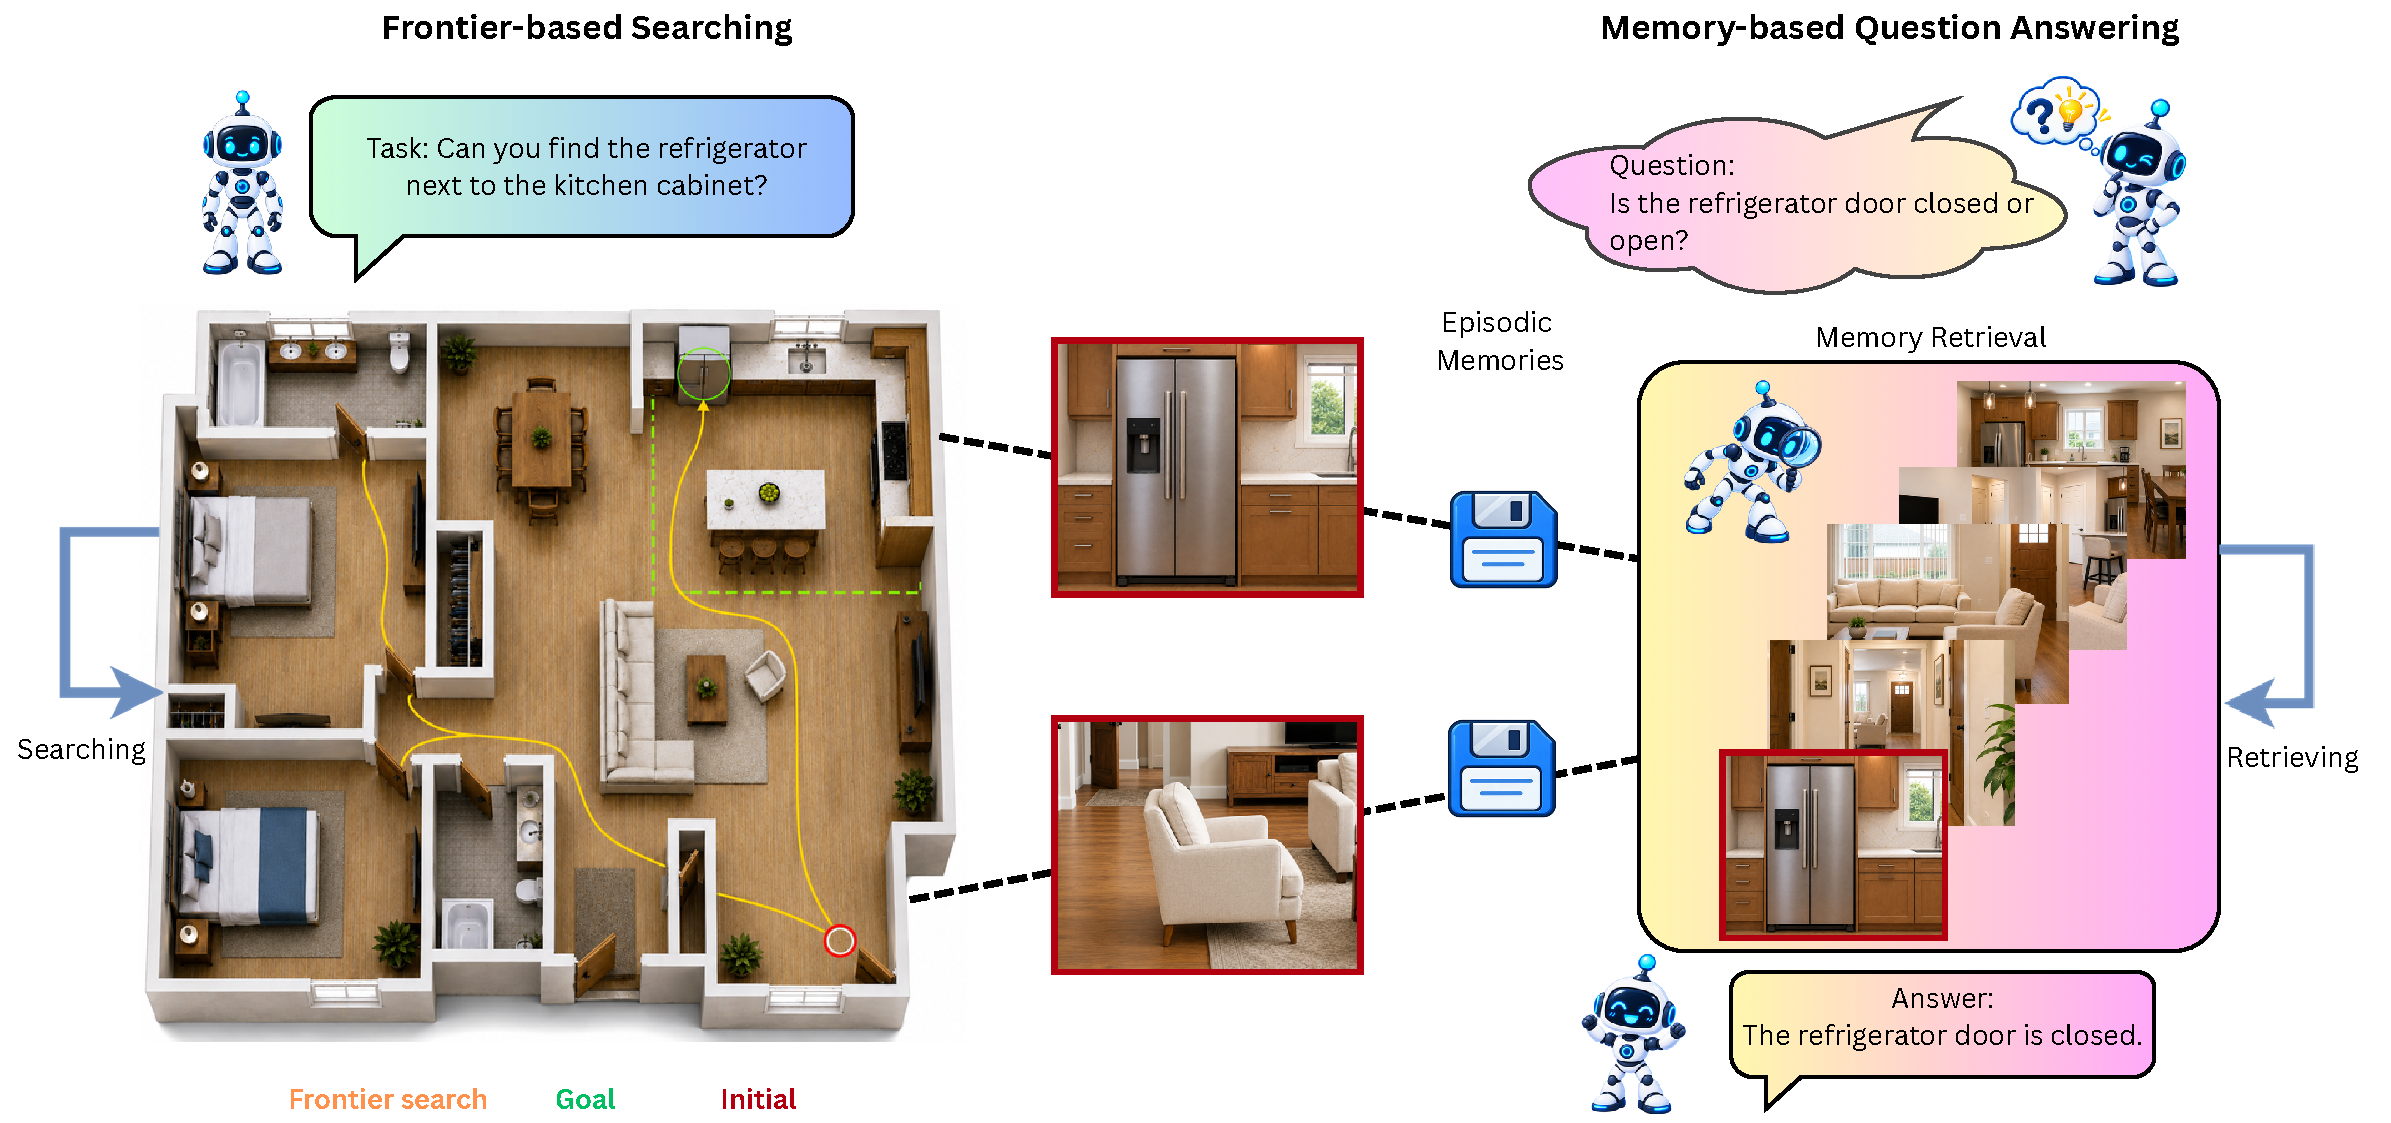
\includegraphics[width=0.92\textwidth]{figures/teaser.pdf}
\caption{\textbf{The EQA problem.} An agent must search an unseen environment by frontier exploration to reach a described target, storing observations as episodic memory, and later answer follow-up questions by retrieving from that memory. What the search fails to observe, retrieval cannot recover.}
\label{fig:teaser}
\end{figure*}

A second opportunity lies in how the task is posed. Long-horizon benchmarks treat every object named in an instruction as a terminal goal. We read them differently. An instruction names its target inside relational context, the rooms it sits in and the objects beside it, and that context is not a disambiguating detail but a prediction of what the agent should encounter. Being already present in the goal descriptions, it requires no annotation and recovers a verification signal that terminal-goal formulations discard.

We use that signal with a simple principle, which is to predict before exploring and then hold those predictions to account. Before moving through a frontier, a Vision-Language Model (VLM)~\cite{bordes2024introduction,feng2025vision,https://doi.org/10.1002/widm.70036,10445007} predicts the semantic layout beyond it from the structured goal, and on arrival the agent measures the divergence from what it observes. This error, not the prediction itself, drives the search. High error broadens exploration and low error narrows it toward the goal, a shift emerging from the error dynamics alone with no schedule and no environment-specific training.

We instantiate this in Predict-Explore-Correct Navigation (PEC-Nav), an EQA pipeline whose search module forms a closed feedback loop (Fig.~\ref{fig:teaser}). An LLM parses the instruction into a target and its relational context, a predictor anticipates the layout beyond each frontier, an uncertainty-aware policy balances goal relevance against prediction confidence, and a correction module updates the predictor's confidence scaling and the explore-exploit weights online. Observations along the way populate an episodic memory that answers follow-up questions, and because memory and QA are fixed across our ablations, changes in answer quality there are attributable to search.

On LMEE-Benchmark dataset official 58-task subset~\cite{wang2026memoryexplorer}, using GPT-4o~\cite{openai2024gpt4o} for goal extraction and search reasoning and Qwen2.5-VL-7B for memory-based question answering, PEC-Nav reaches 24.45\% SR, 16.86 SPL, 57.93 MLLM-Score and 66.21\% QA accuracy.

\paragraph{Our Contributions.}
\begin{enumerate}
    \item We recast the relational context already carried by long-horizon instructions as a verification signal costing no annotation, treating it as a prediction the agent can check against what it observes.
    \item We design the Predict-Explore-Correct loop, to our knowledge the first frontier search to adapt both predictor confidence and explore-exploit weighting online from its own prediction error, within a single episode and with no training.
    \item We build a diagnostic EQA pipeline holding memory and reasoning fixed, isolating search as the experimental variable.
    \item We report gains over a static-search baseline across three ablations, with calibration dynamics read from the correction logs. Our supported claim is path efficiency, since the success-rate differences at this scale are not statistically resolved and we say so throughout.
\end{enumerate}


%%%%%%%%% RELATED WORK
\section{Related Work}

\subsection{Frontier-Based and Zero-Shot Navigation}
\label{sec:related-frontier}

Frontier-based exploration~\cite{yamauchi1997frontier} directs agents toward boundaries between explored and unexplored space, and SemExp~\cite{chaplot2020semexp} learns a goal-conditioned policy over semantic maps. A zero-shot line then replaced learned scorers with pretrained priors, using CLIP~\cite{radford2021clip} and VLM-based frontier evaluation~\cite{gadre2023cow,yokoyama2024vlfm} and injecting LLM common sense to constrain selection~\cite{zhou2023esc}. A second line organises exploration around structured representations, reasoning over 3D scene graphs~\cite{yin2024sgnav} or unifying goal types within one mechanism~\cite{yin2025unigoal}. SCOPE~\cite{wang2026scope} adds potential-based scoring over a spatio-temporal graph with self-reconsideration of earlier decisions.

PEC-Nav is zero-shot in the same sense and adds a feedback path these methods lack. In all of them the scoring function's parameters are fixed for the episode, even where decisions are revisited, so a scorer that is systematically wrong stays wrong. PEC-Nav verifies predictions on arrival and uses the error to retune both predictor confidence and selection weights online. To our knowledge no prior frontier method adapts its scorer within an episode from its own measured prediction error, recovering an adaptivity normally reserved for trained policies.

\subsection{Embodied Question Answering and Memory}

EQA~\cite{das2018eqa} requires agents to gather evidence before answering, and Explore-EQA~\cite{ren2024exploreeqa} showed VLM-guided frontier selection outperforms random exploration. Later work improved reasoning through scene graphs and hybrid exploration~\cite{saxena2025grapheqa,jiang2025fineeqa}, external tools~\cite{wang2025tooleqa}, memory signals fed back to the planner~\cite{zhai2025memorycentric}, and chain-of-view prompting~\cite{cov2026}.

On the memory side, 3D-Mem~\cite{huang20243dmem} builds volumetric spatial memories and MemoryExplorer~\cite{wang2026memoryexplorer} structures episodic memory with spatial-temporal annotations. That work also introduces LMEE-Bench and, as one of its own baselines, RA-Mem, a retrieval-augmented variant of 3D-Mem, which we report under its original name in Table~\ref{tab:lmee}. The benchmark couples multi-goal navigation with memory-based question answering, naming several objects to reach in sequence and afterwards querying the agent about what it observed.

These methods enrich what the agent remembers, but the search deciding what it sees remains governed by a static scorer. Table~\ref{tab:qualitative} sets
out four design dimensions, and the \textbf{Adapt.} column separates PEC-Nav from all of them, since no prior method changes its scorer's parameters
within an episode.


\begin{table}[htbp]
\centering
\caption{\textbf{PEC-Nav vs.\ prior work.} Columns: goal type, mid-episode scorer adaptation, question answering, zero-shot operation; only PEC-Nav has all.}
\label{tab:qualitative}
\vspace{1mm}
\setlength{\tabcolsep}{6pt}
\begin{tabular}{lcccc}
\toprule
\textbf{Method} & \textbf{Goal} & \textbf{Adapt.} & \textbf{QA} & \textbf{ZS} \\
\midrule
SemExp~\cite{chaplot2020semexp}          & Category & $\times$   & $\times$   & $\times$   \\
CoW~\cite{gadre2023cow}                  & Text     & $\times$   & $\times$   & \checkmark \\
ESC~\cite{zhou2023esc}                   & Text     & $\times$   & $\times$   & \checkmark \\
VLFM~\cite{yokoyama2024vlfm}             & Text     & $\times$   & $\times$   & \checkmark \\
Explore-EQA~\cite{ren2024exploreeqa}     & Question & $\times$   & \checkmark & \checkmark \\
SG-Nav~\cite{yin2024sgnav}               & Text     & $\times$   & $\times$   & \checkmark \\
UniGoal~\cite{yin2025unigoal}            & Any      & $\times$   & $\times$   & \checkmark \\
GraphEQA~\cite{saxena2025grapheqa}       & Question & $\times$   & \checkmark & \checkmark \\
Fine-EQA~\cite{jiang2025fineeqa}         & Question & $\times$   & \checkmark & $\times$   \\
ToolEQA~\cite{wang2025tooleqa}           & Question & $\times$   & \checkmark & $\times$   \\
Mem-Centric~\cite{zhai2025memorycentric} & Question & $\times$   & \checkmark & $\times$   \\
SCOPE~\cite{wang2026scope}               & Image    & $\times$   & $\times$   & \checkmark \\
MemExplorer~\cite{wang2026memoryexplorer}& Multi    & $\times$   & \checkmark & \checkmark \\
\midrule
\textbf{PEC-Nav (Ours)}                  & \textbf{Question} & \checkmark & \checkmark & \checkmark \\
\bottomrule
\end{tabular}
\end{table}

%%%%%%%%% METHOD
\section{Method}

Given a natural language prompt, PEC-Nav extracts a structured navigation goal, explores using a self-calibrating frontier search, stores observations in episodic memory, and answers follow-up questions from that memory. Figure~\ref{fig:architecture} gives an overview.

\begin{figure*}[t]
\centering
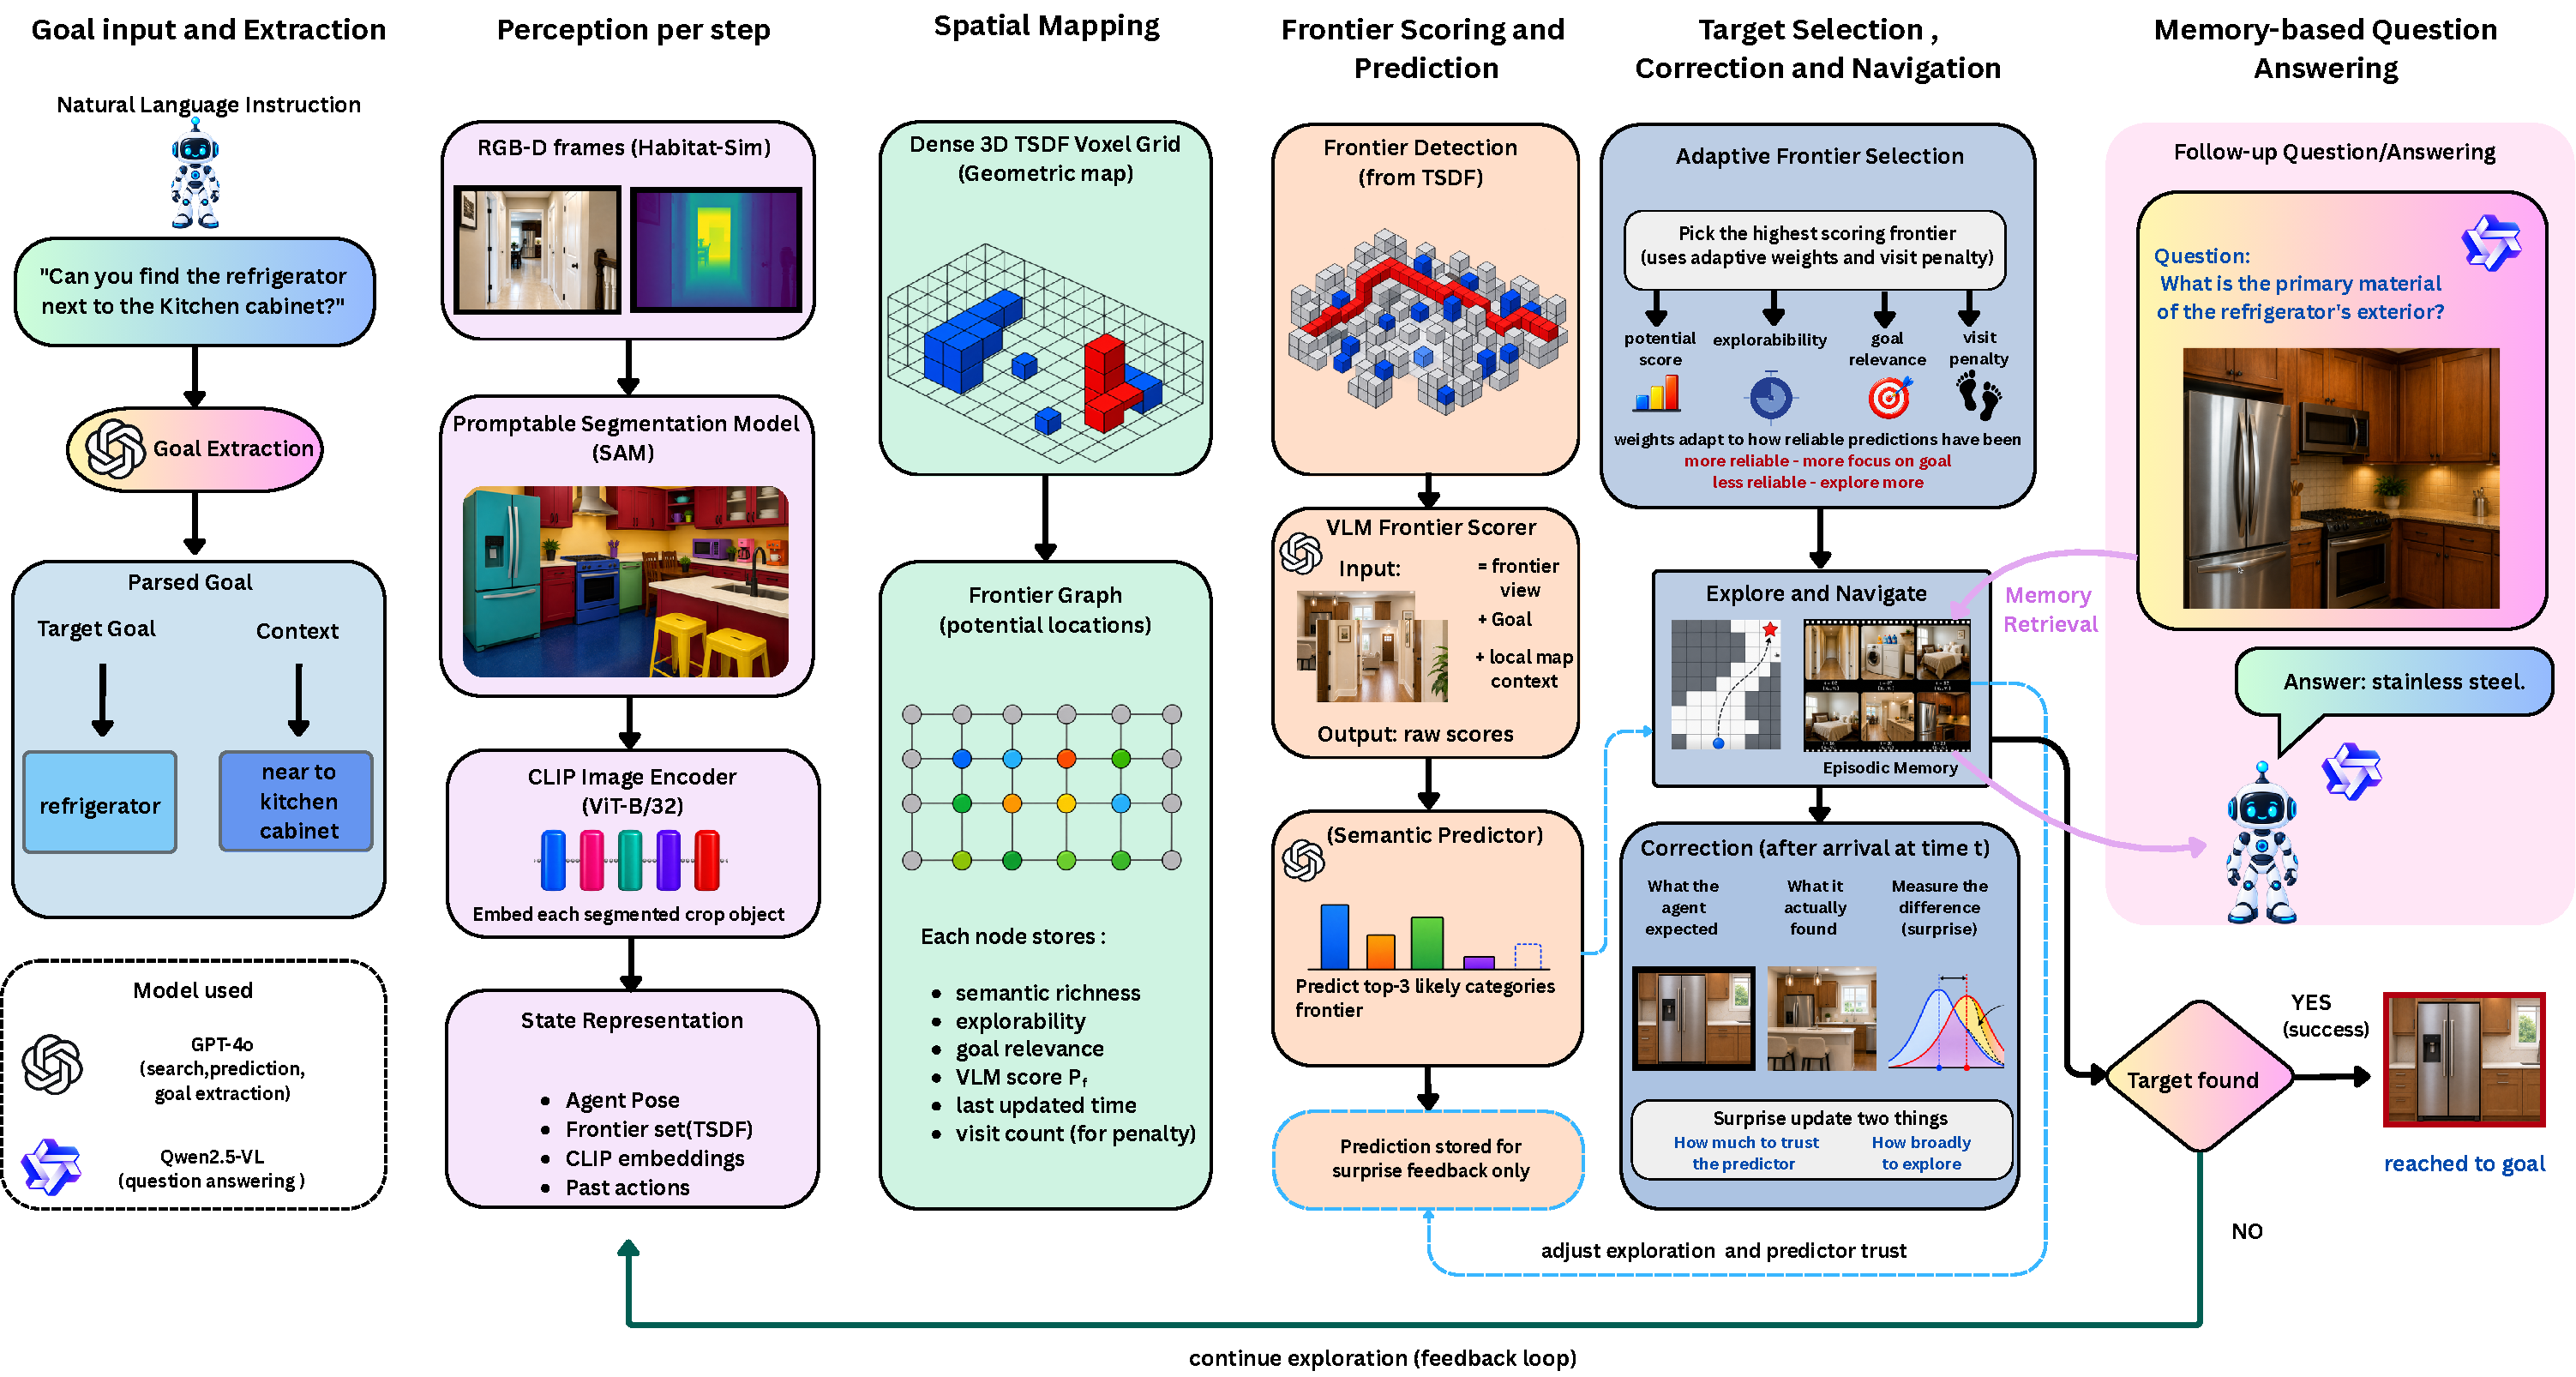
\includegraphics[width=0.93\textwidth]{figures/Pec-main-architecture .pdf}
\caption{\textbf{Illustration of PEC-Nav.} The agent predicts the layout beyond each frontier, selects one, explores it, and corrects the predictor on arrival, and can answer follow-up questions using the episodic memory populated during exploration.}
\label{fig:architecture}
\end{figure*}

\subsection{Goal Extraction}
\label{sec:problem}

Unlike standard ObjectNav, where the goal is a category label or image, our agent receives a natural language prompt such as \emph{``Can you find the refrigerator next to the kitchen cabinet?''}, which carries both spatial context and relational cues. We extract a structured goal using GPT-4o~\cite{openai2024gpt4o}, which receives only the prompt text, with no scene geometry or ground-truth labels, and outputs a \textbf{target category} such as ``refrigerator'' and a \textbf{contextual description} such as ``likely in a kitchen, near cabinets''. This structured goal drives both frontier scoring and semantic prediction throughout the episode.

\subsection{Predict-Explore-Correct Loop}
\label{sec:pec}

The agent fuses egocentric RGB-Depth (RGB-D) observations into a TSDF voxel grid, from which it derives a top-down occupancy map and identifies frontiers as boundaries between explored and unexplored space. Object proposals come from a promptable segmentation model (SAM) and are embedded with a CLIP image encoder~\cite{radford2021clip}, giving the sparse semantic graph over which frontiers are scored. The agent scores each frontier $f$ with a VLM that produces semantic richness ($r_f$), explorability ($e_f$), goal relevance ($g_{r,f}$) and a potential estimate ($p_f$). The four are separate VLM outputs rather than a summary and its parts, and the value function of Sec.~\ref{sec:calibration} uses three of them, with $r_f$ entering only as context for the prompt that produces $p_f$. A frontier scored at step $t'$ and reconsidered at step $t$ carries its score forward discounted by $\gamma^{\,t - t'}$ with $\gamma = 0.95$, so stale assessments lose weight relative to fresh ones. This scoring follows the formulation surveyed in Sec.~\ref{sec:related-frontier} and is not what we contribute, beyond computing goal relevance against our text goal rather than a reference image.

Our contribution is the loop closed around that scorer. One design property is worth stating first. The prediction $\hat{P}_f$ is never a term in $\mathrm{val}(f)$, and its only route into behaviour is the surprise it generates on arrival, which sets $\sigma_t$ and the weights scoring subsequent frontiers. The semantic predictor shapes search by being wrong in a measurable way rather than by voting on the next move.

\paragraph{Prediction.} For each frontier the VLM is prompted with the frontier's egocentric view and the extracted goal, returning the top-3 categories $\{c_1, c_2, c_3\}$ with confidences $\hat{p}_i \in [0,1]$. These are modulated by a self-calibration scale $\sigma_t \in (0.4, 1.0]$ (set by Eq.~\ref{eq:adapt}) and normalised over $C = \{c_1, c_2, c_3, \text{other}\}$,
\begin{align}
    u(c_i) &= \hat{p}_i \, \sigma_t, \quad
    u(\text{other}) = \max\!\left(\epsilon,\, 1 - \textstyle\sum_{i=1}^{3} \hat{p}_i \, \sigma_t\right)
    \label{eq:predict} \\
    \hat{P}(c) &= u(c) \big/ \textstyle\sum_{c' \in C} u(c') . \notag
\end{align}
Normalisation is required rather than cosmetic, since the three confidences need not sum to one and the $\max$ flooring the residual mass can push the total past it. The constant $\epsilon = 10^{-3}$ prevents zero probabilities and also smooths the counts in Eq.~\ref{eq:observed}, regularising both distributions identically. The effect of $\sigma_t$ survives normalisation, since as it falls, mass transfers into the \emph{other} bucket and the agent becomes less committed. Each $\hat{P}_f$ is keyed by the frontier's voxel position and view and scored on arrival as issued rather than rescaled, so surprise measures the error of the belief the agent acted on.

\paragraph{Exploration.} The agent selects $f^* = \arg\max_f \mathrm{val}'(f)$ (Eq.~\ref{eq:calibrate}--\ref{eq:visitpenalty}) and navigates toward it with a point-goal controller, recording egocentric RGB observations into an episodic memory buffer with spatial-temporal coordinates.

\paragraph{Correction.} When the agent comes within $R = 3.0$\,m of a previously predicted frontier, correction fires. The distance is taken on the $(x,z)$ ground plane after transforming the agent's position from the simulator frame to the map frame,
\begin{equation}
    d = \left\lVert \big(w_f^{(x)}, w_f^{(z)}\big) - \big(\mathrm{pts}_{\text{norm}}^{(x)}, \mathrm{pts}_{\text{norm}}^{(z)}\big) \right\rVert_2 ,
    \label{eq:arrival}
\end{equation}
where $w_f$ is the frontier's stored world-frame position and $\mathrm{pts}_{\text{norm}}$ the agent's position after that transform. It then builds an observed distribution over the same support,
\begin{equation}
    Q(c) = \frac{\mathrm{count}(c) + \epsilon}{\sum_{c' \in C} \big(\mathrm{count}(c') + \epsilon\big)} .
    \label{eq:observed}
\end{equation}
These counts come from the Habitat simulator's semantic sensor, so correction consumes privileged information a deployed agent would obtain from a detector, and the accuracy of $Q$ upper-bounds what a detector-based variant would supply. Predict, explore and goal extraction use no ground-truth labels. Restricting both distributions to this small prediction-specific support is what makes the comparison informative, since over a full vocabulary the observation would be near one-hot and the divergence would measure vocabulary sparsity instead of predictive error. The surprise signal is
\begin{equation}
    D_{\mathrm{KL}}(\hat{P} \,\|\, Q) = \sum_{c \in C} \hat{P}(c) \log \frac{\hat{P}(c)}{Q(c)} ,
    \label{eq:kl}
\end{equation}
which is bounded, since flooring both arguments at $\epsilon$ caps any single term at $\log(1/\epsilon) \approx 6.9$ nats. A confident prediction that is fully contradicted therefore produces a large but finite surprise, keeping the signal at the $O(1)$ magnitude the squash below expects.

\subsection{Self-Calibration}
\label{sec:calibration}

Surprise drives two feedback paths through a shared running estimate. We maintain an EMA of per-correction values and squash it to a bounded signal,
\begin{equation}
    \bar{s}_t = (1 - \beta)\,\bar{s}_{t-1} + \beta \, D_{\mathrm{KL}}^{(t)}, \quad
    n_t = 1 - e^{-\bar{s}_t} ,
    \label{eq:ema}
\end{equation}
with $\beta = 0.3$ and $\bar{s}_0 = 0$, an optimistic prior under which the agent trusts its predictions until evidence accumulates. The first path, \textsc{correct-confidence}, scales the predictor's confidence,
\begin{equation}
    \sigma_t = 1 - 0.6\, n_t \in (0.4, 1.0] .
    \label{eq:adapt}
\end{equation}
The regime this produces matters for reading our results. The map is strongly compressive above $\bar{s} \approx 2$, where every value sends $n_t$ into $[0.86, 1)$ and $\sigma_t$ into $(0.4, 0.48]$, so it discriminates sharply among small surprises and barely among large ones, and with $\beta = 0.3$ the EMA reaches it within roughly five corrections. The intent is fast commitment rather than gradual annealing, with the floor bounding how far distrust can go.


\begin{table*}[htbp]
\centering
\caption{\textbf{Results on LMEE-Bench.} Upper block is retrieval-augmented QA over memory banks collected post-exploration, lower block is active exploration.}
\label{tab:lmee}
\footnotesize
\setlength{\tabcolsep}{3pt}
% \begin{tabular}{lcccccccccccccccc}
\begin{tabular}{l|cccc|cccc|cccc|cccc}

\toprule
& \multicolumn{4}{|c}{\textbf{Easy}} & \multicolumn{4}{|c}{\textbf{Medium}} & \multicolumn{4}{|c}{\textbf{Hard}} & \multicolumn{4}{|c}{\textbf{Total}} \\
\cmidrule(lr){2-5} \cmidrule(lr){6-9} \cmidrule(lr){10-13} \cmidrule(lr){14-17}
& \multicolumn{2}{c}{Nav} & \multicolumn{2}{c|}{QA} & \multicolumn{2}{c}{Nav} & \multicolumn{2}{c|}{QA} & \multicolumn{2}{c}{Nav} & \multicolumn{2}{c|}{QA} & \multicolumn{2}{c}{Nav} & \multicolumn{2}{c}{QA} \\
\cmidrule(lr){2-3} \cmidrule(lr){4-5} \cmidrule(lr){6-7} \cmidrule(lr){8-9} \cmidrule(lr){10-11} \cmidrule(lr){12-13} \cmidrule(lr){14-15} \cmidrule(lr){16-17}
\textbf{Method} & SR & SPL & Score & Acc & SR & SPL & Score & Acc & SR & SPL & Score & Acc & SR & SPL & Score & Acc \\
\midrule
\multicolumn{17}{l}{\emph{Retrieval-Augmented QA}} \\
LLaVA-OneVision-7B~\cite{li2024llavaov} & N/A & N/A & 35.71 & 57.14 & N/A & N/A & 42.02 & 62.77 & N/A & N/A & 25.00 & 43.75 & N/A & N/A & 38.62 & 59.31 \\
Llama3.2-Vision-11B & N/A & N/A & 43.57 & 48.57 & N/A & N/A & 28.19 & 37.23 & N/A & N/A & 20.31 & 31.25 & N/A & N/A & 31.03 & 39.31 \\
Qwen2.5-VL-7B & N/A & N/A & 36.43 & 65.71 & N/A & N/A & 43.62 & 53.19 & N/A & N/A & 42.19 & 43.75 & N/A & N/A & 41.72 & 55.17 \\
InternVL3-8B & N/A & N/A & 42.14 & 65.71 & N/A & N/A & 41.22 & 54.26 & N/A & N/A & 26.56 & 43.75 & N/A & N/A & 39.83 & 55.86 \\
Qwen3-VL-8B~\cite{bai2025qwen3} & N/A & N/A & 43.57 & 65.71 & N/A & N/A & 36.70 & 58.51 & N/A & N/A & 32.81 & 62.50 & N/A & N/A & 37.93 & 60.69 \\
GPT-4o~\cite{openai2024gpt4o} & N/A & N/A & 43.57 & 65.71 & N/A & N/A & 37.50 & 51.06 & N/A & N/A & 40.62 & 56.25 & N/A & N/A & 39.31 & 55.17 \\
Gemini-2.5-Flash & N/A & N/A & 44.29 & 51.43 & N/A & N/A & 37.77 & 50.00 & N/A & N/A & 23.44 & 50.00 & N/A & N/A & 37.76 & 50.34 \\
\midrule
\multicolumn{17}{l}{\emph{MLLM Exploration}} \\
Explore-EQA~\cite{ren2024exploreeqa} & 4.26 & 4.26 & N/A & N/A & 15.17 & 8.67 & N/A & N/A & 14.89 & 7.25 & N/A & N/A & 13.24 & 7.66 & N/A & N/A \\
3D-Mem~\cite{huang20243dmem} & 21.28 & 9.68 & 30.71 & 42.86 & 15.73 & 6.09 & 34.57 & 44.68 & 17.02 & 6.97 & 25.00 & 18.75 & 16.91 & 6.86 & 32.59 & 41.38 \\
RA-Mem$^{\ddagger}$~\cite{wang2026memoryexplorer} & 25.53 & 15.65 & 34.29 & 54.29 & \textbf{21.35} & 12.14 & 37.77 & 62.77 & 14.89 & 8.86 & 25.00 & 43.75 & 20.96 & 12.18 & 35.52 & 58.62 \\
MemoryExplorer~\cite{wang2026memoryexplorer} & 31.91 & 21.11 & 35.71 & \textbf{68.57} & \textbf{21.35} & 14.03 & 48.14 & 63.83 & 23.40 & 12.51 & 34.38 & \textbf{68.75} & 23.53 & 14.99 & 43.62 & 65.52 \\
\midrule
\textbf{PEC-Nav (Ours)} & \textbf{40.43} & \textbf{25.06} & \textbf{48.57} & \textbf{68.57} & 20.11 & \textbf{14.35} & \textbf{62.77} & \textbf{67.02} & \textbf{25.00} & \textbf{18.21} & \textbf{50.00} & 56.25 & \textbf{24.45} & \textbf{16.86} & \textbf{57.93} & \textbf{66.21} \\
\bottomrule
\end{tabular}
\end{table*}

The second path, \textsc{correct-weights}, shifts the value function along the explore-exploit spectrum,
\begin{align}
    \mathrm{val}(f) &= w_p \, p_f + w_e \, e_f + w_g \, g_{r,f} \label{eq:calibrate} \\
    w_p &= 0.5, \quad w_e = 0.3 + 0.2\,n_t, \quad w_g = 0.2 - 0.2\,n_t , \notag
\end{align}
with weights summing to one for all $n_t$. Under sustained surprise $w_e$ reaches 0.5 and $w_g$ falls to zero, so selection is carried by how much unexplored potential a frontier offers rather than by how well it matches the goal. This makes $w_g$ the most aggressively scheduled term, and whether a nonzero floor on it would serve better is untested. A soft visit penalty then discourages unproductive revisitation,
\begin{equation}
    \mathrm{val}'(f) = \mathrm{val}(f) \cdot \max\!\left(0.1, \; \frac{1}{1 + 0.5 \cdot \mathrm{visits}(f)}\right) ,
    \label{eq:visitpenalty}
\end{equation}
where the floor of 0.1 keeps repeatedly visited frontiers from being scored out entirely.

Algorithm~\ref{alg:pecnav} summarises the decision cycle.

\begin{algorithm}[htbp]
\caption{PEC-Nav decision cycle}
\label{alg:pecnav}
\begin{algorithmic}[1]
\REQUIRE Frontiers $\mathcal{F}$, goal $g$, state $(\sigma_t, n_t, \bar{s}_t)$
\ENSURE Selected frontier $f^*$, updated state
\FOR{each $f \in \mathcal{F}$}
    \STATE $p_f, e_f, g_{r,f} \leftarrow \text{VLMScore}(f, g)$
    \STATE $\hat{P}_f \leftarrow \text{PredictLayout}(f, g, \sigma_t)$ \COMMENT{Eq.~\ref{eq:predict}, stored not scored}
    \STATE $\mathrm{val}'(f) \leftarrow$ Eq.~\ref{eq:calibrate}--\ref{eq:visitpenalty}
\ENDFOR
\STATE $f^* \leftarrow \arg\max_{f} \mathrm{val}'(f)$, navigate toward $f^*$
\IF{$d(f') \le R$ for any previously-predicted $f'$}
    \STATE $Q \leftarrow \text{ObservedLayout}(f')$ \COMMENT{Eq.~\ref{eq:observed}}
    \STATE $\bar{s}_t \leftarrow (1{-}\beta)\bar{s}_{t-1} + \beta \, D_{\mathrm{KL}}(\hat{P}_{f'} \| Q)$
    \STATE $n_t \leftarrow 1 - e^{-\bar{s}_t}$, \quad $\sigma_t \leftarrow 1 - 0.6 n_t$, \quad update $w_e, w_g$
\ENDIF
\end{algorithmic}
\end{algorithm}

\subsection{Memory, QA and Implementation}
\label{sec:memory}

Every egocentric RGB observation is stored with spatial-temporal coordinates, and follow-up questions are answered by retrieving and reasoning over them. Across our ablations memory and QA are held identical with only search varying, so changes in answer quality there are attributable to search. This does not extend to the published rows of Table~\ref{tab:lmee}, whose memory modules differ.

Question answering runs locally on a Qwen2.5-VL-7B model, with the full protocol in Sec.~\ref{sec:setup}. Table~\ref{tab:hyperparams} lists all hyperparameters, tuned on 5 development scenes and then fixed.

\begin{table}[htbp]
\centering
\caption{PEC-Nav hyperparameters. $\dagger$ marks an inherited default.}
\label{tab:hyperparams}
\footnotesize
\setlength{\tabcolsep}{4pt}
\begin{tabular}{@{}llll@{}}
\toprule
\textbf{Symbol} & \textbf{Value} & \textbf{Symbol} & \textbf{Value} \\
\midrule
$\gamma^\dagger$ & 0.95 & $w_p$ & 0.5 (fixed) \\
$\epsilon$ & $10^{-3}$ & $w_e$ & $[0.3, 0.5]$ \\
$R$ & 3.0\,m & $w_g$ & $[0.0, 0.2]$ \\
$\beta$ & 0.3 & $\sigma_t$ & $(0.4, 1.0]$ \\
$\bar{s}_0$ & 0 & Visit disc., floor & 0.5,\; 0.1 \\
\bottomrule
\end{tabular}
\end{table}



%%%%%%%%% EXPERIMENTS
\section{Experiments}

We evaluate PEC-Nav through four analyses. A contextual positioning against published results, ablations isolating each component and each feedback path, a direct measurement of calibration behaviour, and an analysis of cost and failure modes.

\subsection{Setup}
\label{sec:setup}

\paragraph{Dataset.} All experiments use LMEE-Benchmark dataset official 58-task evaluation subset~\cite{wang2026memoryexplorer}, comprising 32 HM3D scenes, 274 navigation goals and 145 QA questions, stratified into easy, medium and hard by region count, goal count and distance. We adopt the benchmark unchanged and use its Qwen2.5-VL-7B~\cite{bai2025qwen25vl} QA model as our backend, which holds the answering stage constant across our ablations so differences there originate in what search delivered. It does not make our pipeline equivalent to the reference system, whose memory module differs.

\paragraph{Units and metrics.} An episode is one LMEE-Benchmark dataset~\cite{wang2026memoryexplorer} task containing several navigation subtasks, one per goal in its instruction, giving 274 subtasks over 58 episodes. Navigation metrics are per subtask, so every $N$ below counts subtasks. Success Rate (\textbf{SR}) is the fraction reaching the target within 1.0\,m, and Success weighted by Path Length (\textbf{SPL})~\cite{anderson2018spl} weights success by path efficiency on a 0 to 100 scale. Open-ended answers use \textbf{MLLM-Score}~\cite{wang2026memoryexplorer}, multiple choice uses \textbf{accuracy}. An episode is a success if all its subtasks succeed, partial if some do, and fail if none. Instrumentation coverage differs by analysis, with correction logs retained for 29 episodes and failure logs for 36 across 19 scenes, so figures drawn from them describe the mechanism rather than the full set.

\paragraph{Protocol.} Goal extraction and search reasoning use GPT-4o~\cite{openai2024gpt4o} via API. Memory-based question answering runs locally on the benchmark's own Qwen2.5-VL-7B~\cite{bai2025qwen25vl} model in bf16 on a single NVIDIA RTX 3090, loaded only for QA subtasks. Search reasoning depends on a hosted model versioned outside our control, so reproduction requires the same snapshot and we report single runs. Comparison rows are quoted from the benchmark paper and assume its protocol and step budget, treating an instruction's named objects as successive subtasks. Our counts recover 274 subtasks against 272 for those rows, so per-split percentages are comparable to within roughly 0.4 points and no finer.

\subsection{Comparison on the LMEE-Benchmark dataset}

\begin{table*}[htbp]
\centering
\caption{\textbf{Results on the LMEE-Benchmark dataset.} Upper block is retrieval-augmented QA over memory banks collected post-exploration, lower block is active exploration.}
\label{tab:lmee}
\footnotesize
\setlength{\tabcolsep}{3pt}
\begin{tabular}{l|cccc|cccc|cccc|cccc}
\toprule
& \multicolumn{4}{|c}{\textbf{Easy}} & \multicolumn{4}{|c}{\textbf{Medium}} & \multicolumn{4}{|c}{\textbf{Hard}} & \multicolumn{4}{|c}{\textbf{Total}} \\
\cmidrule(lr){2-5} \cmidrule(lr){6-9} \cmidrule(lr){10-13} \cmidrule(lr){14-17}
& \multicolumn{2}{c}{Nav} & \multicolumn{2}{c|}{QA} & \multicolumn{2}{c}{Nav} & \multicolumn{2}{c|}{QA} & \multicolumn{2}{c}{Nav} & \multicolumn{2}{c|}{QA} & \multicolumn{2}{c}{Nav} & \multicolumn{2}{c}{QA} \\
\cmidrule(lr){2-3} \cmidrule(lr){4-5} \cmidrule(lr){6-7} \cmidrule(lr){8-9} \cmidrule(lr){10-11} \cmidrule(lr){12-13} \cmidrule(lr){14-15} \cmidrule(lr){16-17}
\textbf{Method} & SR & SPL & Score & Acc & SR & SPL & Score & Acc & SR & SPL & Score & Acc & SR & SPL & Score & Acc \\
\midrule
\multicolumn{17}{l}{\emph{Retrieval-Augmented QA}} \\
LLaVA-OneVision-7B~\cite{li2024llavaov} & N/A & N/A & 35.71 & 57.14 & N/A & N/A & 42.02 & 62.77 & N/A & N/A & 25.00 & 43.75 & N/A & N/A & 38.62 & 59.31 \\
Llama3.2-Vision-11B & N/A & N/A & 43.57 & 48.57 & N/A & N/A & 28.19 & 37.23 & N/A & N/A & 20.31 & 31.25 & N/A & N/A & 31.03 & 39.31 \\
Qwen2.5-VL-7B~\cite{bai2025qwen25vl} & N/A & N/A & 36.43 & 65.71 & N/A & N/A & 43.62 & 53.19 & N/A & N/A & 42.19 & 43.75 & N/A & N/A & 41.72 & 55.17 \\
InternVL3-8B & N/A & N/A & 42.14 & 65.71 & N/A & N/A & 41.22 & 54.26 & N/A & N/A & 26.56 & 43.75 & N/A & N/A & 39.83 & 55.86 \\
Qwen3-VL-8B~\cite{bai2025qwen3} & N/A & N/A & 43.57 & 65.71 & N/A & N/A & 36.70 & 58.51 & N/A & N/A & 32.81 & 62.50 & N/A & N/A & 37.93 & 60.69 \\
GPT-4o~\cite{openai2024gpt4o} & N/A & N/A & 43.57 & 65.71 & N/A & N/A & 37.50 & 51.06 & N/A & N/A & 40.62 & 56.25 & N/A & N/A & 39.31 & 55.17 \\
Gemini-2.5-Flash & N/A & N/A & 44.29 & 51.43 & N/A & N/A & 37.77 & 50.00 & N/A & N/A & 23.44 & 50.00 & N/A & N/A & 37.76 & 50.34 \\
\midrule
\multicolumn{17}{l}{\emph{MLLM Exploration}} \\
Explore-EQA~\cite{ren2024exploreeqa} & 4.26 & 4.26 & N/A & N/A & 15.17 & 8.67 & N/A & N/A & 14.89 & 7.25 & N/A & N/A & 13.24 & 7.66 & N/A & N/A \\
3D-Mem~\cite{huang20243dmem} & 21.28 & 9.68 & 30.71 & 42.86 & 15.73 & 6.09 & 34.57 & 44.68 & 17.02 & 6.97 & 25.00 & 18.75 & 16.91 & 6.86 & 32.59 & 41.38 \\
RA-Mem$^{\ddagger}$~\cite{wang2026memoryexplorer} & 25.53 & 15.65 & 34.29 & 54.29 & \textbf{21.35} & 12.14 & 37.77 & 62.77 & 14.89 & 8.86 & 25.00 & 43.75 & 20.96 & 12.18 & 35.52 & 58.62 \\
MemoryExplorer~\cite{wang2026memoryexplorer} & 31.91 & 21.11 & 35.71 & \textbf{68.57} & \textbf{21.35} & 14.03 & 48.14 & 63.83 & 23.40 & 12.51 & 34.38 & \textbf{68.75} & 23.53 & 14.99 & 43.62 & 65.52 \\
\midrule
\textbf{PEC-Nav (Ours)} & \textbf{40.43} & \textbf{25.06} & \textbf{48.57} & \textbf{68.57} & 20.11 & \textbf{14.35} & \textbf{62.77} & \textbf{67.02} & \textbf{25.00} & \textbf{18.21} & \textbf{50.00} & 56.25 & \textbf{24.45} & \textbf{16.86} & \textbf{57.93} & \textbf{66.21} \\
\bottomrule
\end{tabular}
\end{table*}

Table~\ref{tab:lmee} places PEC-Nav among results from the available literature, reporting MLLM-Score for open-ended answers and accuracy for multiple choice, with bold marking the best value per column and N/A a metric a method does not produce. Navigation columns are compared over the exploration block, since retrieval-augmented methods answer from memory banks collected beforehand and perform no navigation. RA-Mem~\cite{wang2026memoryexplorer}, marked $\ddagger$, is a retrieval-augmented variant of 3D-Mem~\cite{huang20243dmem} introduced as a baseline alongside the benchmark. On the \emph{Total} column it reaches 24.45\% SR, 16.86 SPL, 57.93 MLLM-Score and 66.21\% QA accuracy, ahead of MemoryExplorer~\cite{wang2026memoryexplorer} on SR, SPL and MLLM-Score. The largest per-column margin is MLLM-Score on \emph{Hard} at 50.00 against 34.38, followed by \emph{Medium}. The picture is not uniform. MemoryExplorer retains the better SR on \emph{Medium} and the better QA accuracy on \emph{Hard}, where Qwen3-VL-8B~\cite{bai2025qwen3} also exceeds us, and Easy and Total QA accuracy read as ties. The gains are therefore in navigation and open-ended answer quality rather than multiple-choice accuracy, where the fixed QA module dominates.

\subsection{Ablation Studies}
\label{sec:ablations}

\begin{table}[htbp]
\centering
\caption{\textbf{Feedback-path ablation} over 47 navigation subtasks.}
\label{tab:feedback}
\footnotesize
\setlength{\tabcolsep}{3pt}
\begin{tabular}{@{}l|cc|ccc@{}}
\toprule
\textbf{Variant} & $\sigma_t$ & $w_e,w_g$ & \textbf{SR} $\uparrow$ & \textbf{SPL} $\uparrow$ & $\Delta$\textbf{SR} \\
\midrule
No correction & \xmark & \xmark & 36.17 \,\scriptsize(17/47) & 20.75 & --- \\
Confidence only & \cmark & \xmark & 40.43 \,\scriptsize(19/47) & 25.57 & +4.26 \\
Reweighting only & \xmark & \cmark & 36.17 \,\scriptsize(17/47) & 22.09 & +0.00 \\
\textbf{Full PEC loop} & \cmark & \cmark & \textbf{40.43} \,\scriptsize(19/47) & \textbf{28.38} & \textbf{+4.26} \\
\bottomrule
\end{tabular}
\end{table}

\paragraph{Isolating the correction phase.} The first and last rows of Table~\ref{tab:feedback} differ only in whether arrival detection fires. With correction disabled the predictor still runs and predictions are still stored, but surprise is never computed, so $\sigma_t$ never updates and the weights never shift, leaving the agent with strictly more computation and no adaptation. Enabling correction raises SR from 36.17\% to 40.43\% and SPL from 20.75 to 28.38.

In absolute terms the SR change is 17 successes against 19, and the two proportions are indistinguishable on an unpaired reading, with Wilson 95\% intervals of $[24.0, 50.5]$ and $[27.6, 54.7]$ and Fisher exact $p = 0.83$. The design is paired, but we did not log per-subtask outcome pairs and so decline to quote McNemar's test. The 37\% relative gain in SPL is the more informative number, and does not depend on a success threshold. One subtask is worth 2.13 SR points at $N = 47$ and 4.17 at $N = 24$.

\begin{table}[htbp]
\centering
\caption{\textbf{Component ablation} over 24 navigation subtasks, with success counts in parentheses.}
\label{tab:ablation_all}
\footnotesize
\setlength{\tabcolsep}{3pt}
\begin{tabular}{@{}l|cccc@{}}
\toprule
\textbf{Configuration} & \textbf{SR (\%)} $\uparrow$ & \textbf{SPL} $\uparrow$ & \textbf{N} & $\Delta$\textbf{SR} \\
\midrule
Static baseline & 54.17 \,\scriptsize(13/24) & 34.35 & 24 & --- \\
\quad + Goal extraction & 54.17 \,\scriptsize(13/24) & 36.05 & 24 & 0.00 \\
\quad + Semantic predictor & 50.00 \,\scriptsize(12/24) & 32.36 & 24 & $-$4.17 \\
\quad \textbf{+ Online correction (full)} & \textbf{58.33} \,\scriptsize(14/24) & \textbf{41.47} & 24 & \textbf{+4.16} \\
\bottomrule
\end{tabular}
\end{table}

\paragraph{Component ablation.} Table~\ref{tab:ablation_all} adds each component cumulatively over a separate 2-scene subset, where one subtask is worth 4.17 SR points and the SPL column therefore carries more of the signal. Absolute values are not comparable with Table~\ref{tab:feedback}, since the static baseline scores 54.17 here against 36.17 there, so these rows are within-table contrasts only. Goal extraction leaves SR unchanged and lifts SPL from 34.35 to 36.05. Adding the semantic predictor then moves SR by $-4.17$ and SPL by $-3.69$, which indicates that an uncalibrated predictor steers the agent toward frontiers matching its prediction rather than the observation. Correction recovers that loss and clears the baseline, moving SR by $+8.33$ and SPL by $+9.11$ over the predictor-only row. Within this table the gain is therefore attributable to the loop rather than the predictor, though at $N = 24$ that remains a hypothesis the data are consistent with.

\paragraph{Which feedback path carries the effect.} Surprise rescales predictor confidence through $\sigma_t$ and reweights the value function through $w_e$ and $w_g$. Table~\ref{tab:feedback} enables each independently over a 47-subtask ablation subset, and every nonzero SR difference in it is two subtasks. Confidence scaling recovers the full SR gain alone, while reweighting leaves SR unchanged and lifts SPL from 20.75 to 22.09. The full loop matches confidence-only on SR and extends SPL to 28.38, so reweighting contributes path efficiency rather than successes. Both arms succeed on 19 of 47 subtasks, and we have not verified they are the same 19, which is a further reason to read this table from its SPL column.

\subsection{Does the Agent Calibrate?}
\label{sec:pec-dynamics}

This section asks whether the mechanism behaves as claimed, using quantities from the correction logs.

\begin{figure}[htbp]
\centering
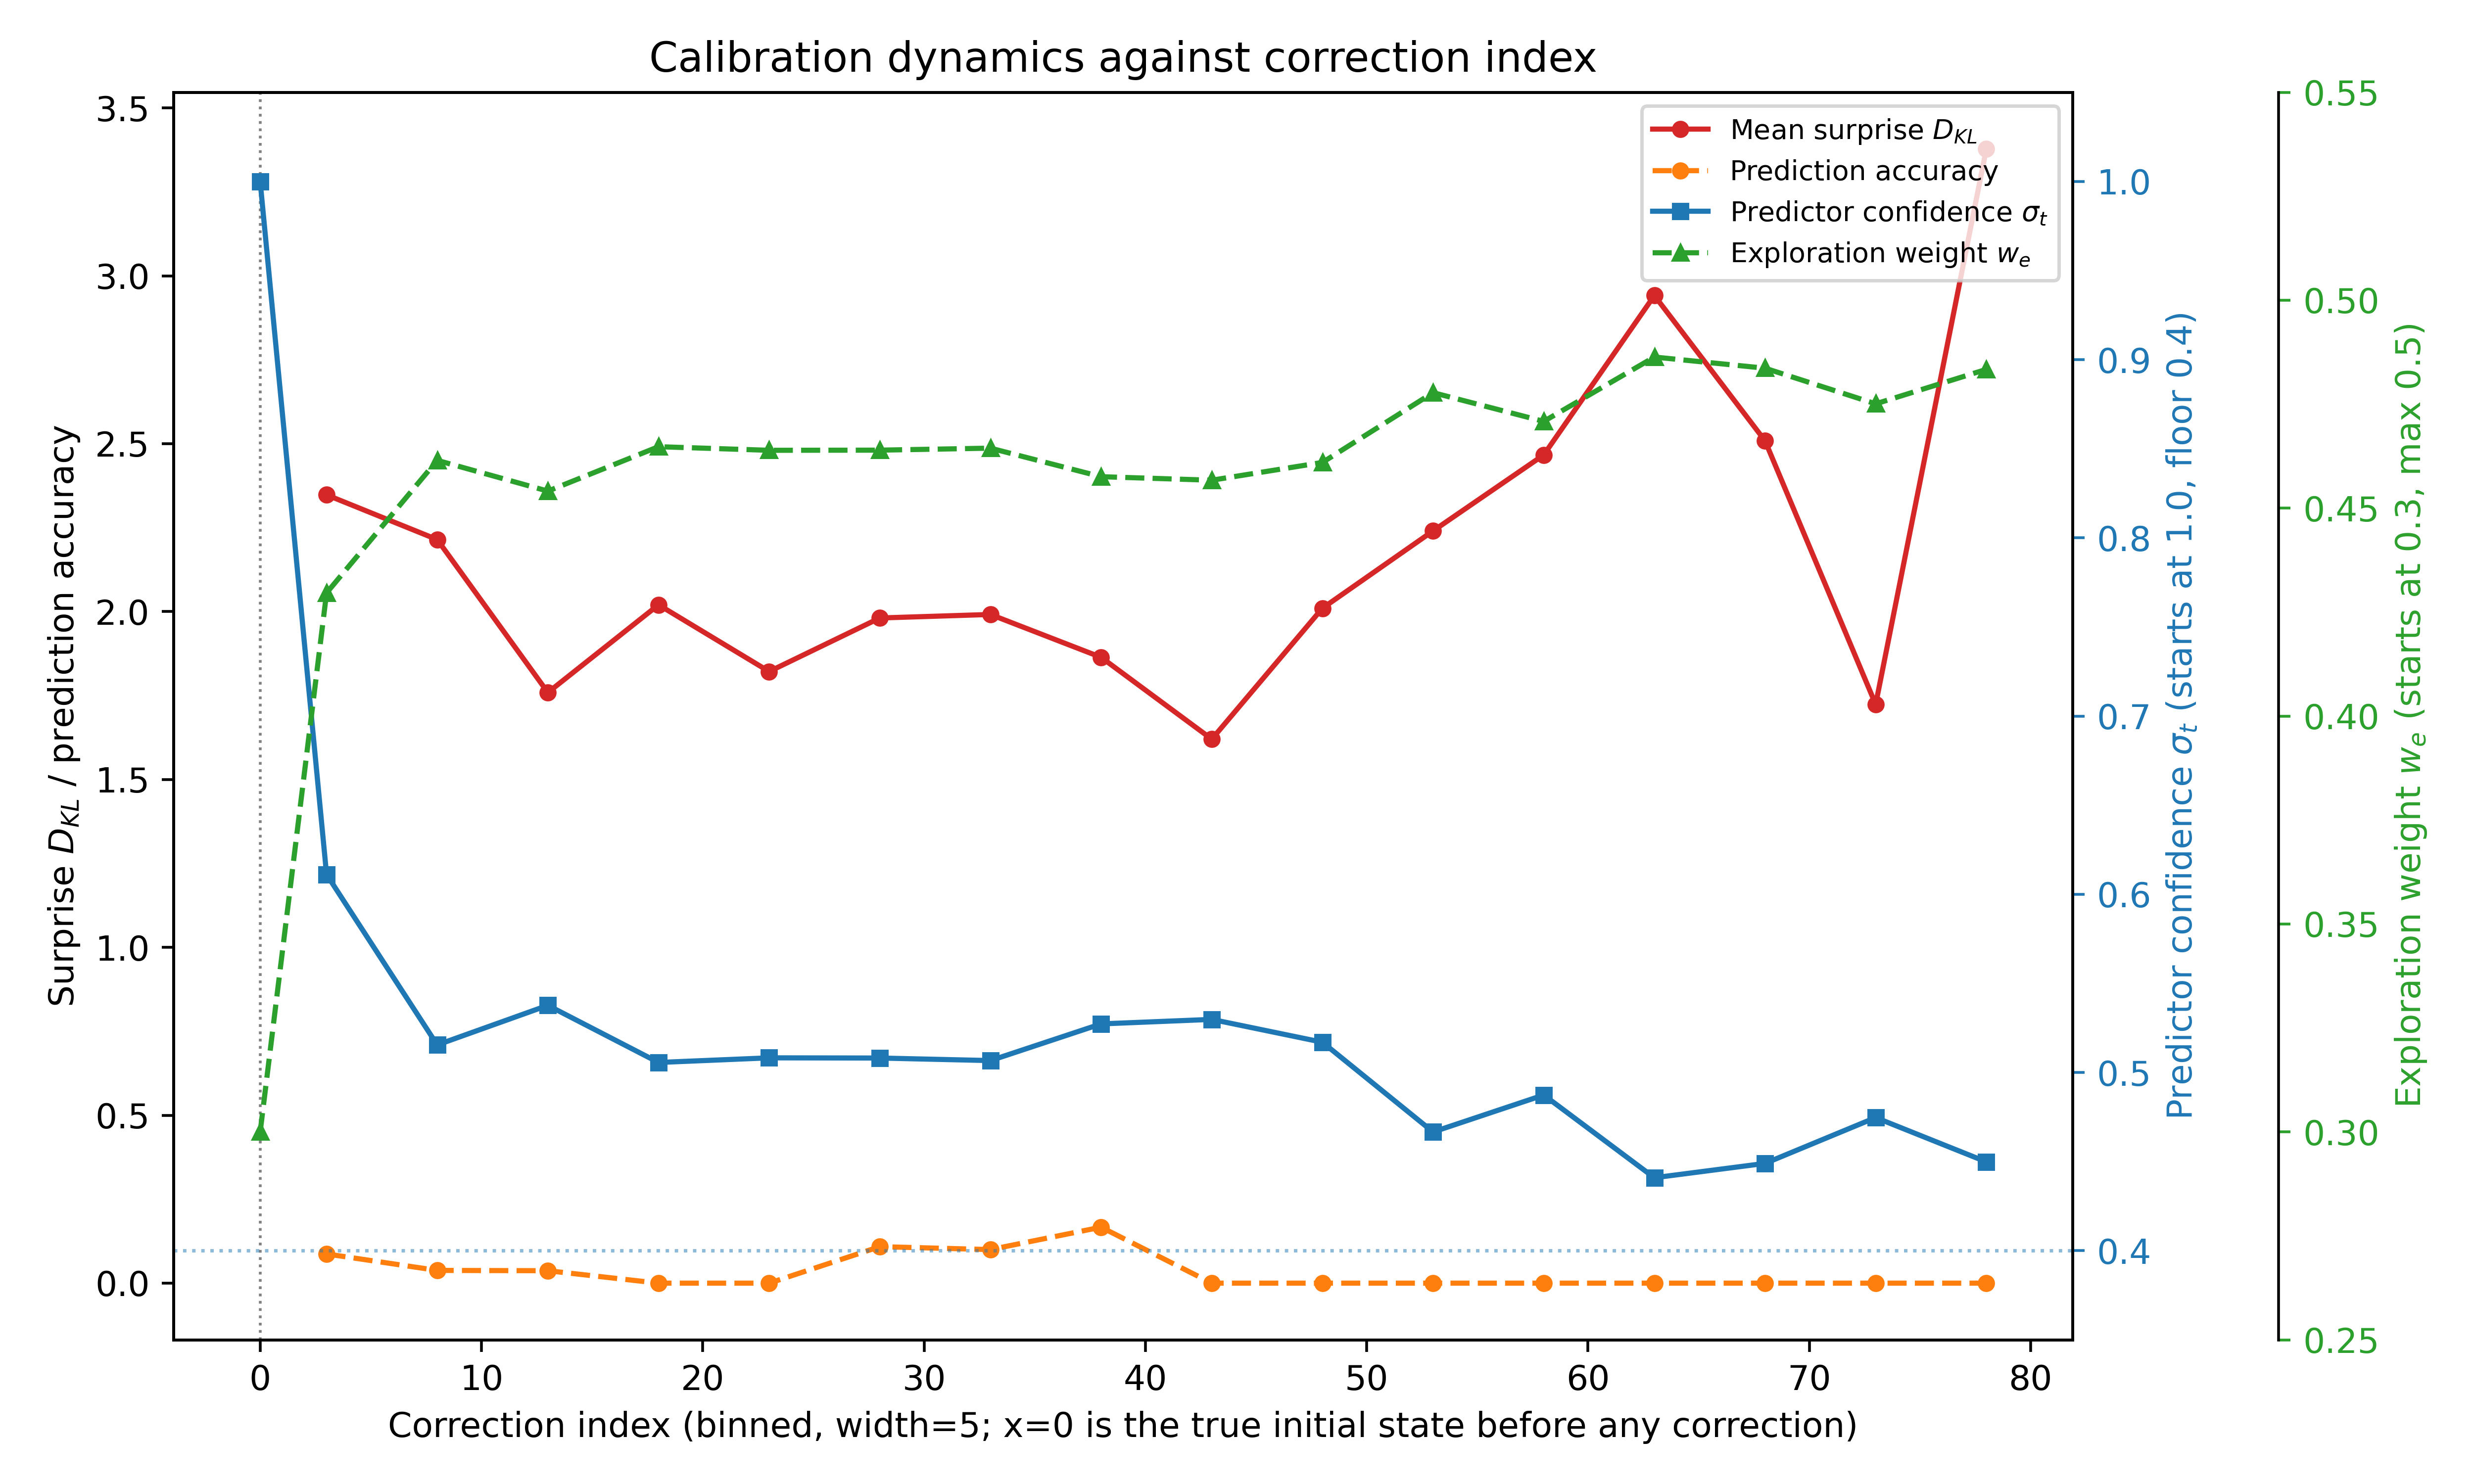
\includegraphics[width=0.88\linewidth]{figures/figure3.png}
\caption{Calibration dynamics: surprise, accuracy, uncertainty vs.\ correction index.}
\label{fig:calibration}
\end{figure}

The regime is the one the self-calibration design anticipates. Per-episode mean divergence is of order $2$, which puts $n_t$ near $0.86$ and $\sigma_t$ within roughly $0.08$ of its floor for most of an episode, so the controller commits quickly to a low-trust setting and holds there. Figure~\ref{fig:calibration} confirms this, with $\sigma_t$ falling and $w_e$ rising under sustained surprise. Neither surprise nor accuracy is expected to improve, since the predictor is never updated and the loop's role is to downweight it.

\begin{figure*}[htbp]
\centering
\includegraphics[width=0.85\textwidth]{figures/qualitative image pec .pdf}
\caption{\textbf{Qualitative examples of PEC-Nav.}}
\label{fig:qualitative}
\end{figure*}


\begin{figure}[htbp]
\centering
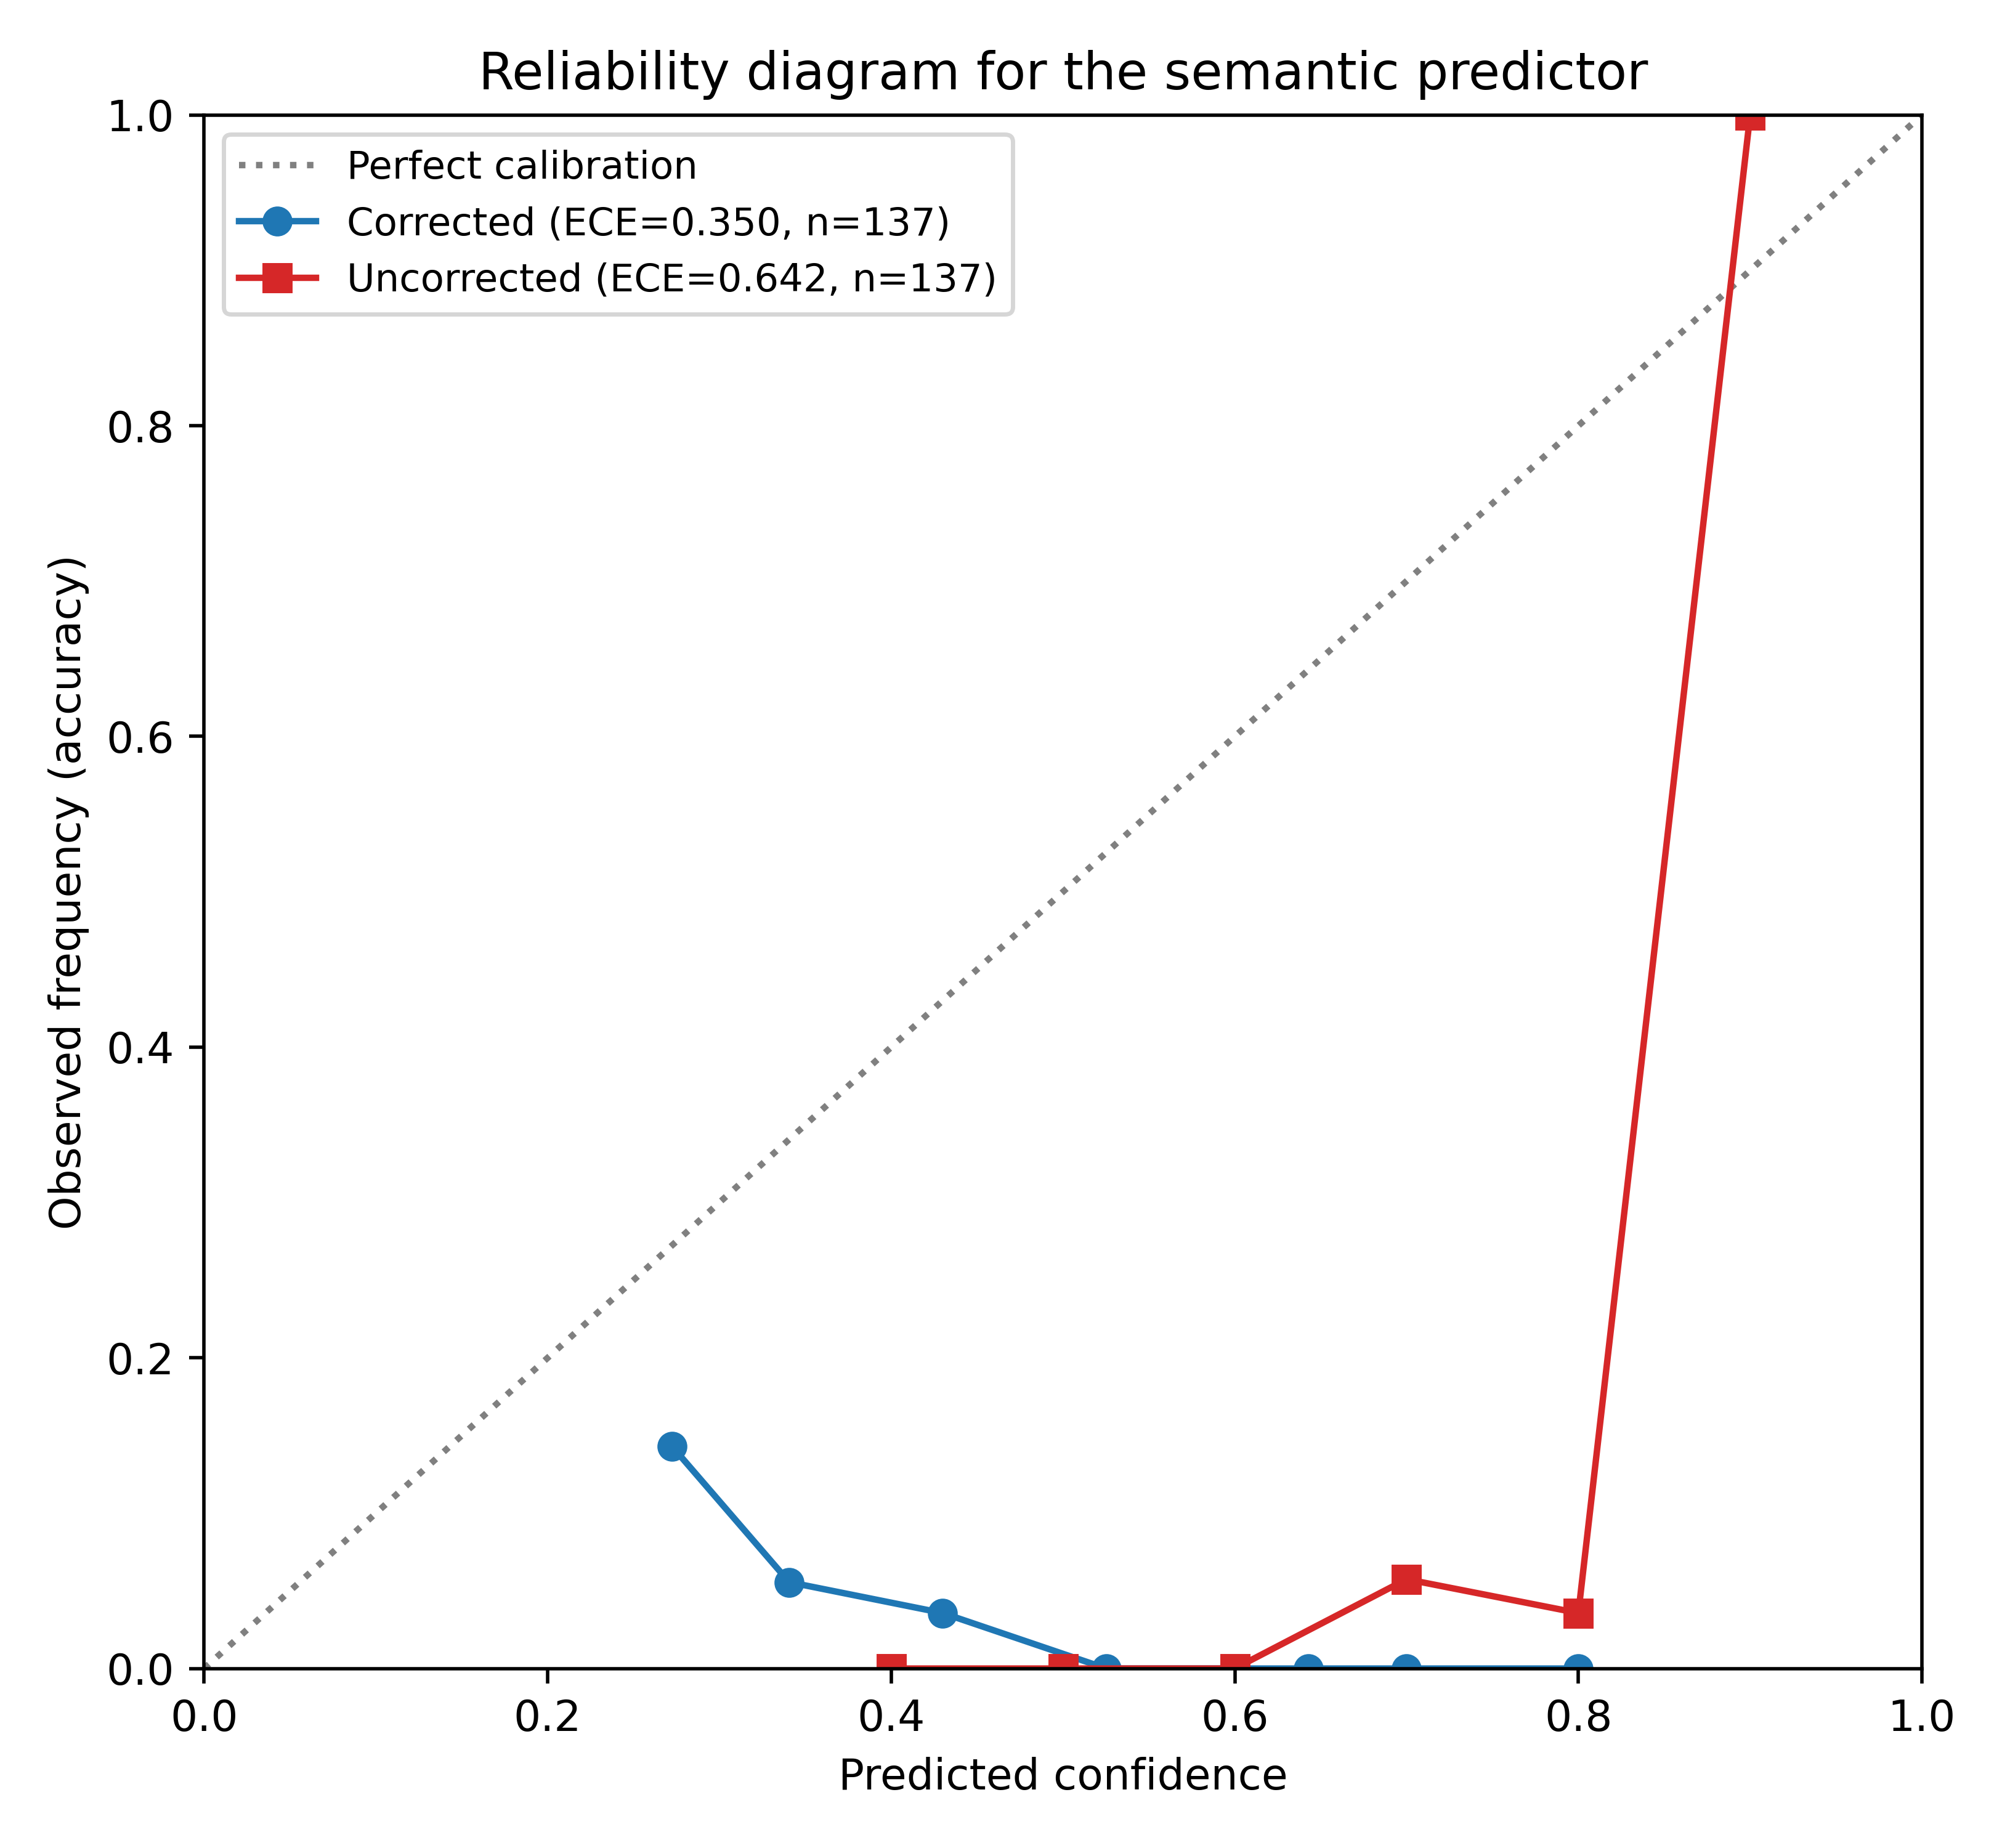
\includegraphics[width=0.75\linewidth]{figures/figure4.png}
\caption{Reliability diagram, with/without correction loop ($n=137$); ECE drops from $0.642$ to $0.350$.}
\label{fig:reliability}
\end{figure}

Figure~\ref{fig:reliability} makes the claim quantitative, and expected calibration error falls from $0.642$ to $0.350$. We are deliberate about what this shows. Since $\sigma_t$ is a multiplicative shrinkage on a systematically overconfident predictor, any downward rescaling moves the metric the same way, and the mechanism is self-referential in that the same $\sigma_t$ enters the divergence driving it. The figure establishes that the loop selects a shrinkage improving calibration without supervision, not that it beats a well-chosen constant, a control we did not run.

\subsection{Analysis}
\label{sec:analysis}

\paragraph{Surprise as a diagnostic.} Across the 29 episodes with retained correction logs, per-episode mean surprise is comparable between partial ($2.10$, $n = 13$) and failed ($1.92$, $n = 16$) episodes. That subset contains no fully successful episode, so the comparison that would matter most cannot be made on it. Surprise aggregated to the episode level is therefore not a reliable diagnostic, and the within-episode dynamics remain the operative signal.

\begin{table}[htbp]
\centering
\caption{\textbf{Cost of the correction loop}, per-episode averages, 4-scene subset.}
\label{tab:compute}
\footnotesize
\setlength{\tabcolsep}{3pt}
\begin{tabular}{@{}l|cc@{}}
\toprule
\textbf{Quantity (per episode)} & \textbf{Static baseline} & \textbf{PEC-Nav} \\
\midrule
VLM calls            & 144.1  & 227.7 \\
Navigation steps     & 100.3  & 95.6 \\
Wall-clock (s)       & 765.09 & 1160.92 \\
Peak GPU memory (GB) & 22.62  & 22.62 \\
\bottomrule
\end{tabular}
\end{table}

\paragraph{Cost of the loop.} Table~\ref{tab:compute} reports the loop's cost on the 4-scene subset, raising VLM calls by 58\% and wall-clock time by 52\%, borne almost entirely in hosted-API calls. The 83.6 extra calls per episode exceed the roughly 30 corrections fired, because each step prices a prediction for every open frontier, not only the one later verified. Peak GPU memory is unchanged, since only the shared local QA model occupies it, and navigation steps fall, so the added cost is deliberation rather than travel, which is also why SPL improves while compute rises. We report no compute figures for the comparison systems, so we claim only that the overhead is a bounded inference-time cost requiring no training and no additional local hardware.

\begin{figure}[htbp]
\centering
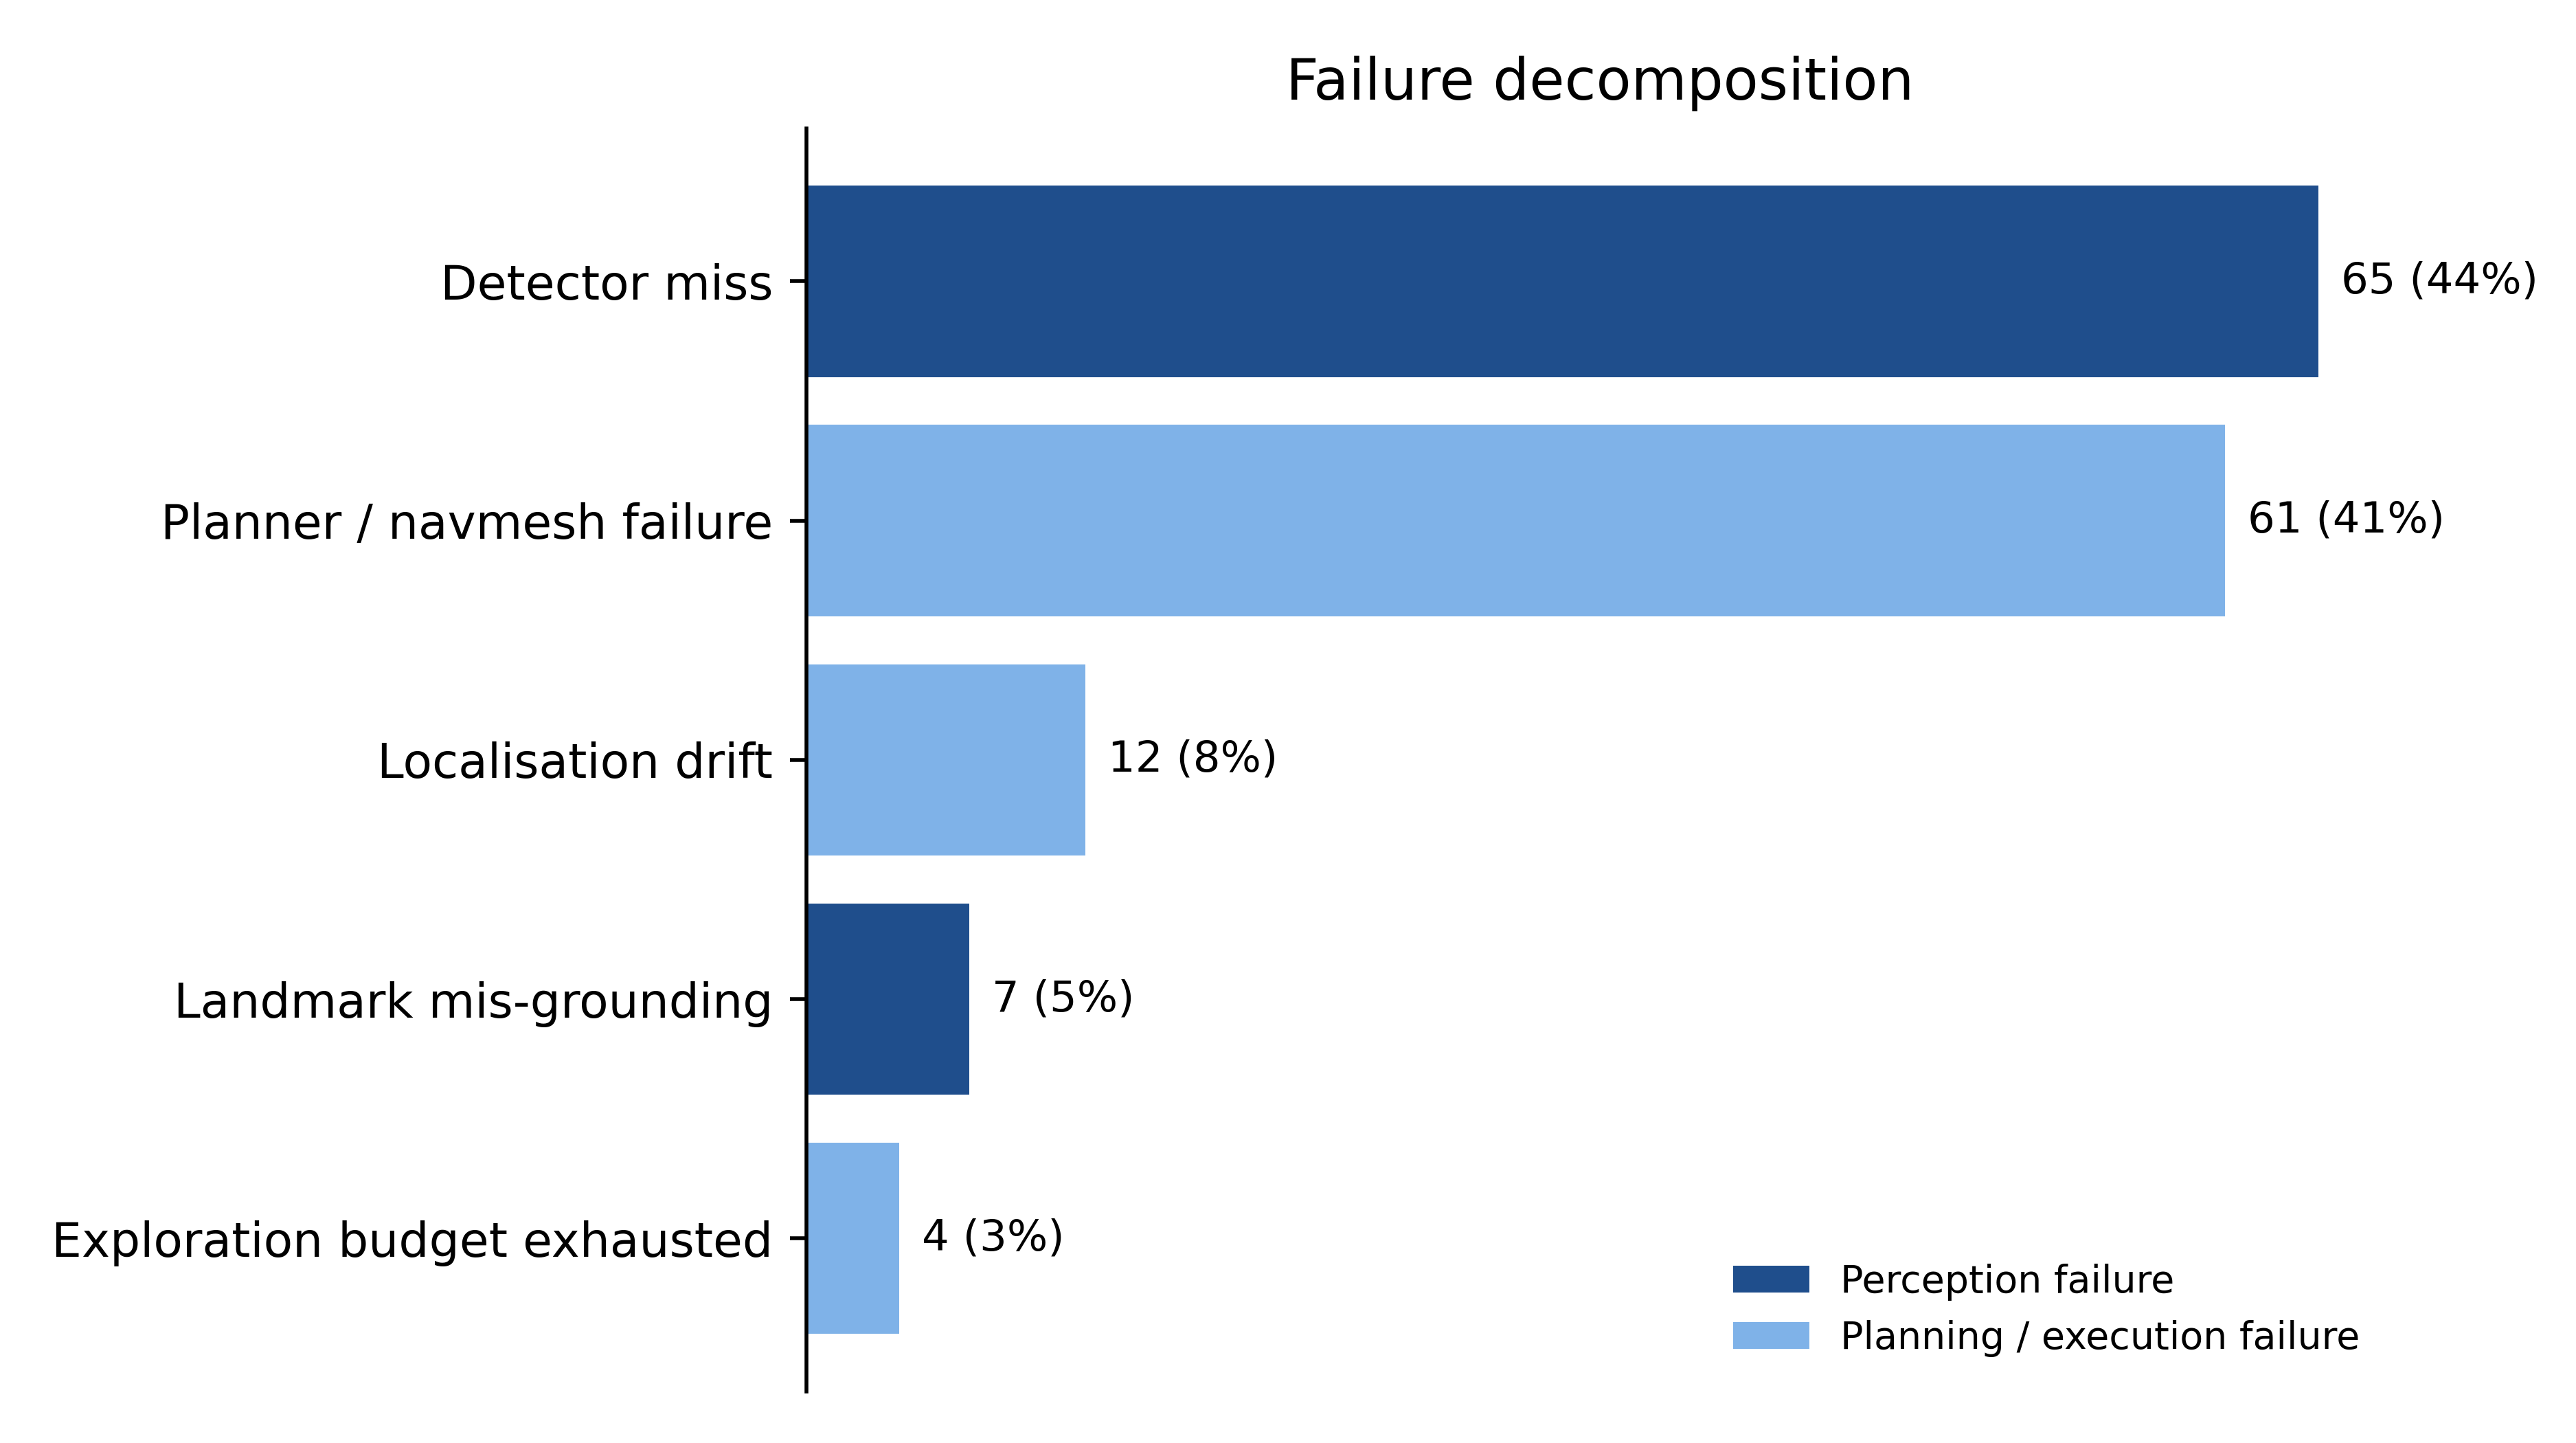
\includegraphics[width=0.88\linewidth]{figures/figure5.png}
\caption{\textbf{Failure decomposition.} By cause across $n=149$ logged records covering 19 of 32 scenes. Percentages are rounded independently and need not total 100.}
\label{fig:failures}
\end{figure}
\paragraph{Where it fails.} Figure~\ref{fig:failures} decomposes the logged subtask failures by cause, and two dominate. Detector misses account for 65 and planner or navmesh failures for 61, together 85\% of the total. Neither is addressable by better frontier selection, which bounds how much any search-side contribution can move the headline number. Figure~\ref{fig:qualitative} shows a trajectory in which surprise is high from the first corrections, the controller drops $\sigma_t$ toward its floor, and the search stays broad thereafter.



%%%%%%%%% Discusiion
\section{Discussion}
\label{sec:discussion}

Every controlled comparison points the same way, with correction improving both metrics in Table~\ref{tab:feedback} and the same ordering on a different subset in Table~\ref{tab:ablation_all}. The literature comparison is not evidence here, since it has no loop-disabled row. What isolation we have comes from 47 and 24 subtasks, where one subtask moves SR by 2.13 and 4.17 points, so no individual delta is resolved and the case rests on SPL and on consistency of direction.

The decomposition locates the effect, with confidence scaling carrying the SR change and reweighting contributing only path efficiency. The finding we consider most interesting is that the predictor alone is a net negative and becomes useful only once something verifies it. Two properties bound how far this carries. Search reasoning depends on a hosted API, tying results to a snapshot outside our control, and the correction phase reads its observed distribution from the simulator's semantic sensor rather than a detector.


%%%%%%%%% CONCLUSION
\begin{figure}[htbp]
\centering
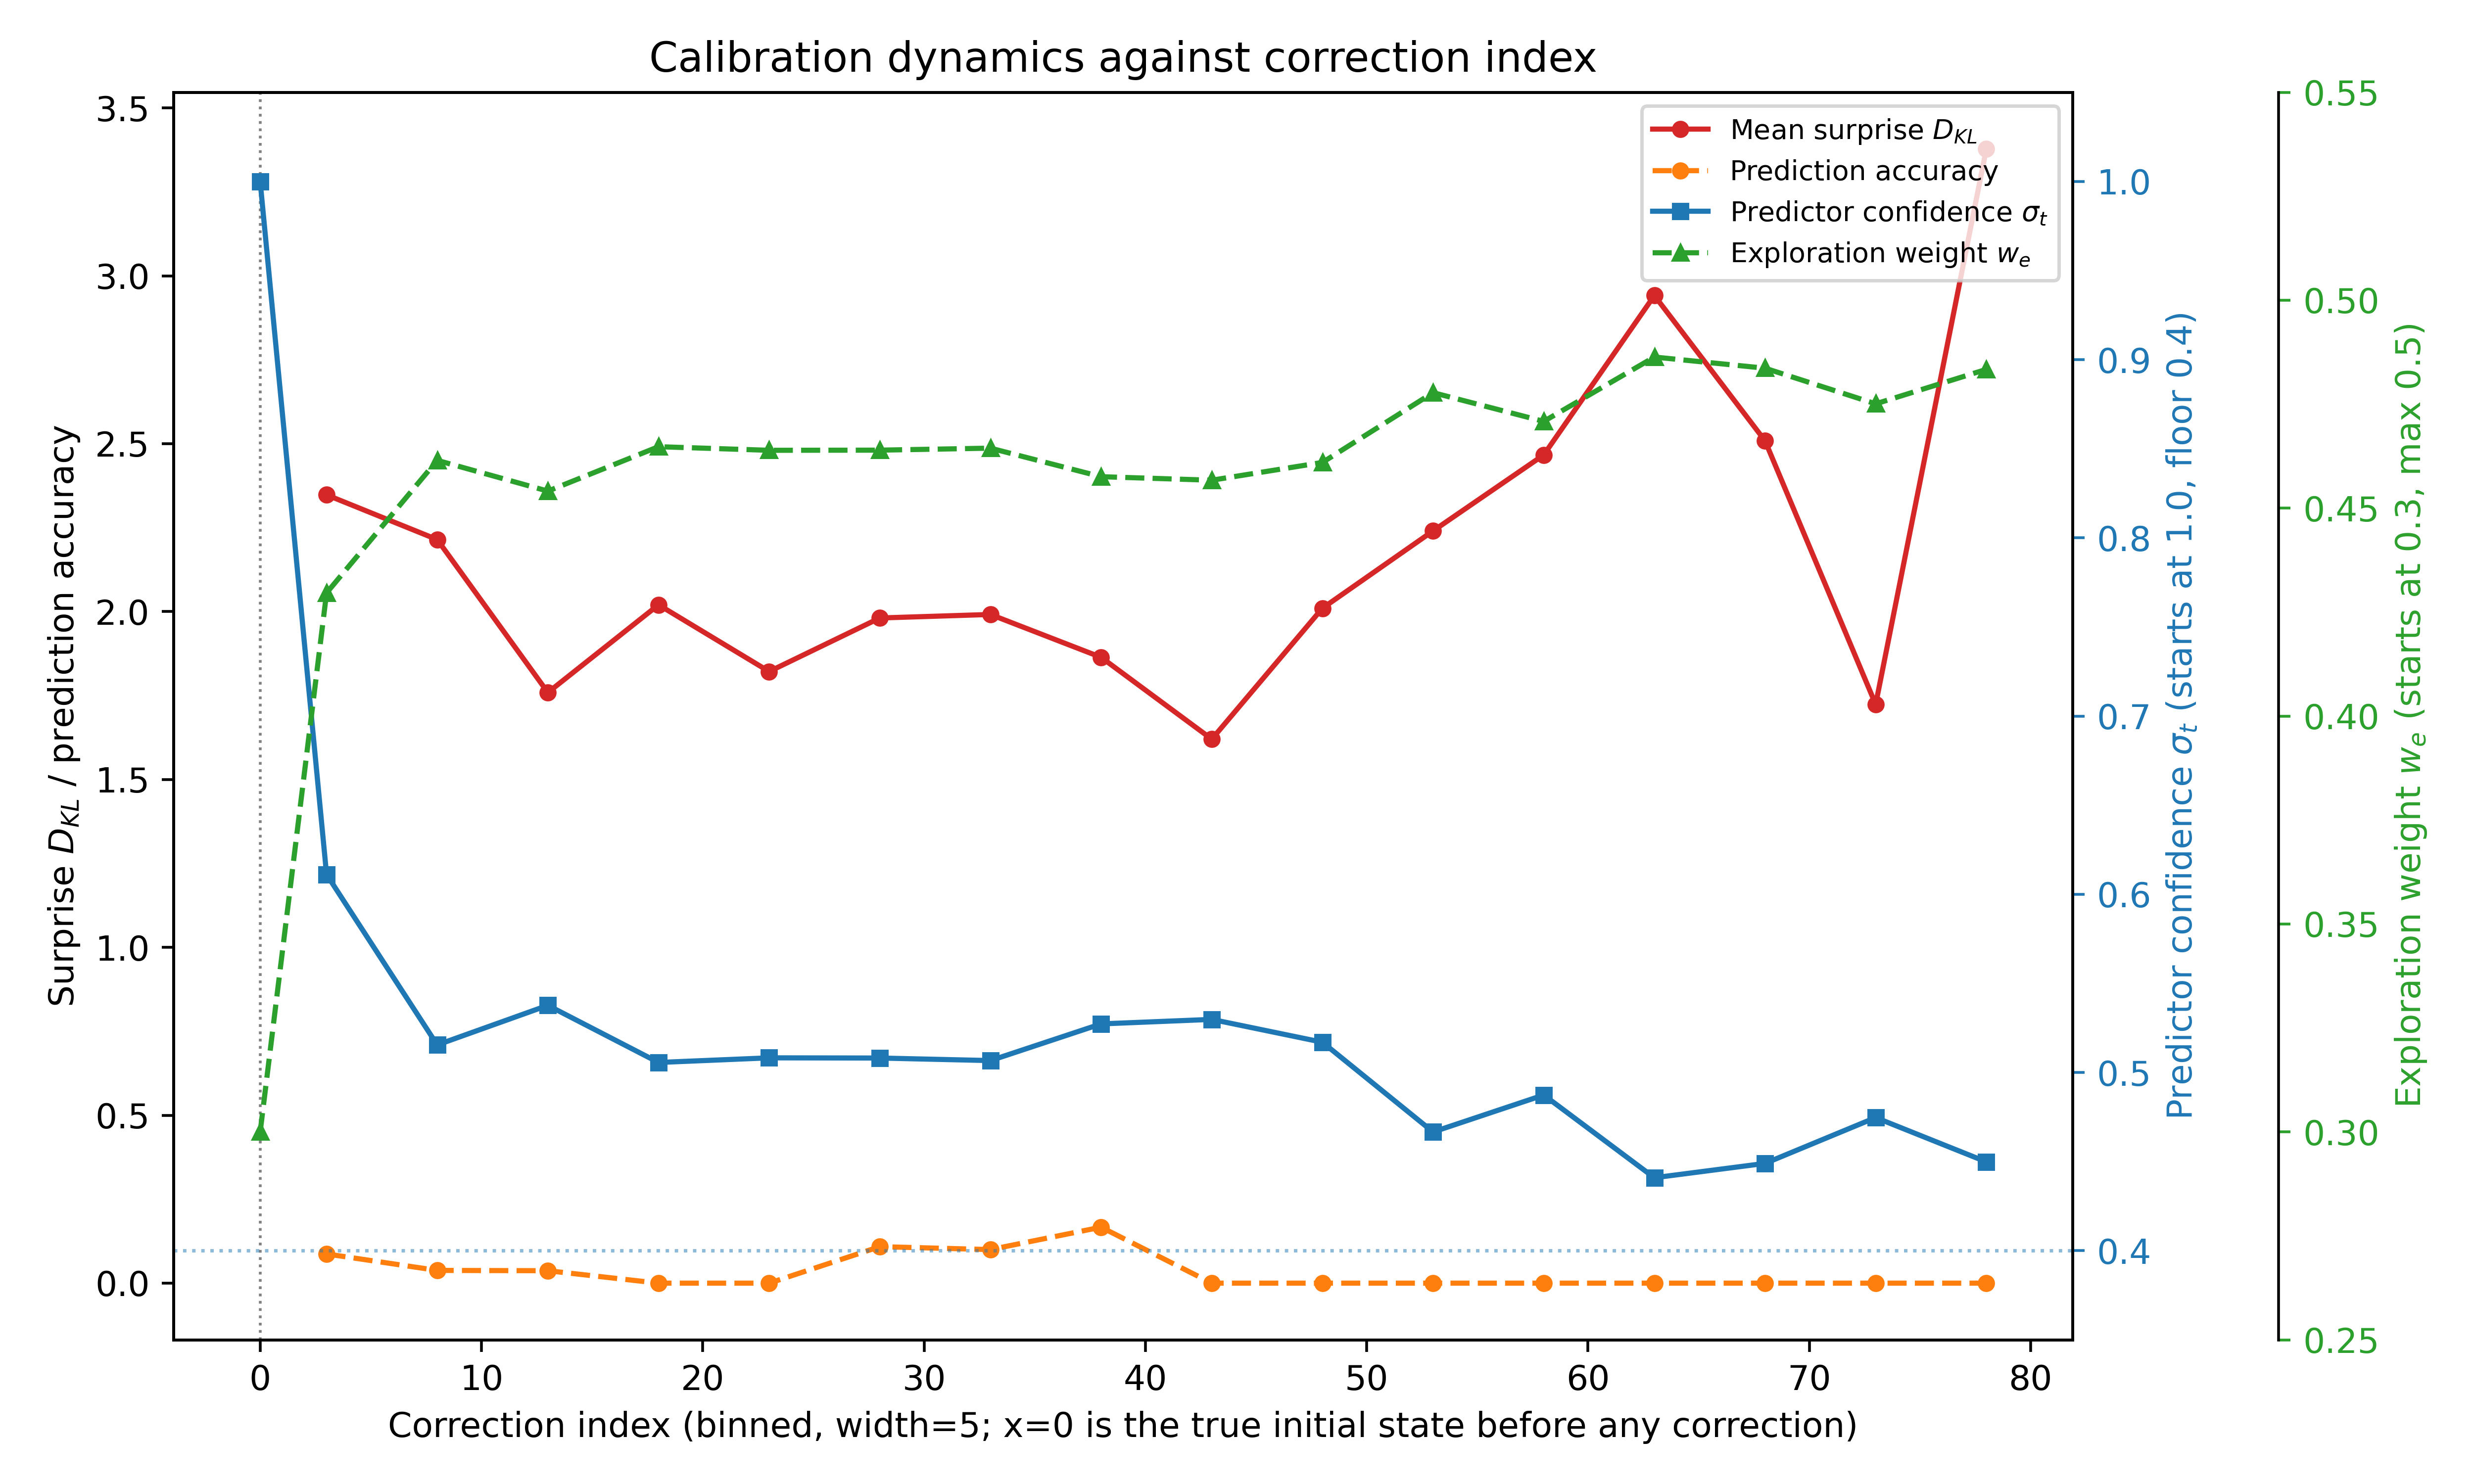
\includegraphics[width=0.88\linewidth]{figures/figure3.png}
\caption{Calibration dynamics: surprise, accuracy, uncertainty vs. correction index}
\label{fig:calibration}
\end{figure}
\section{Conclusion}

We introduced PEC-Nav, a self-calibrating frontier search for embodied question answering. The insight is that prediction errors are more useful than predictions, since measuring surprise between anticipated and observed layouts lets the agent adapt its confidence and exploration balance within an episode, untrained. On LMEE-Bench's 58-task subset it reaches 24.45\% SR, 16.86 SPL, 57.93 MLLM-Score and 66.21\% QA accuracy, and across three ablations the loop improves success and path efficiency while the predictor alone does not. The evidence is directional rather than resolved. Next steps include a learned detector in place of the semantic sensor, a fixed-scalar control separating calibration from shrinkage, and a static baseline at full scale.


%%%%%%%%% REFERENCES
{\small
\bibliographystyle{ieee_fullname}
\bibliography{references}
}

\end{document}
